\chapter{椭圆曲线密码学与配对}\label{chap:15}

在前面的章节中,我们看到了离散对数、CDH 和 DDH 假设在有限循环群 $\mathbb{G}$ 中的许多应用。对于这样的群 $\mathbb{G}$,我们的一个常用的例子是整数的乘法群(或其子群),其中的模数 $p$ 是一个足够大的素数。这个群——由于一些原因——是有问题的,最明显的是,这个群上的离散对数问题不够困难。我们将在第\ref{chap:17}章中讨论的一个最知名的算法,称为\textbf{普通数域筛选法 (general number field sieve, GNFS)},它的运行时间为 $\exp(\tilde O((\log p)^{1/3}))$。在2019年,这种方法被用来解决一个 $795$ 比特素数的离散对数问题。这就是为什么在实践中,我们必须使用长度至少为 $2048$ 比特的素数 $p$ 的原因。高安全性的应用必须使用更大的素数,但这种大素数的模算术运算速度很慢,大大增加了部署使用该群的密码系统的成本。

其他几个明显具有离散对数难度的有限循环群族也相继被提出。在所有这些提案中,有限域上的椭圆曲线点群是最适合实践的,并且在今天的互联网上被广泛地使用。目前,对于大小为 $q$ 的椭圆曲线群,最好的离散对数算法也需要 $O(\sqrt{q})$ 的运行时间。这意味着,想要提供与 AES-128 相当的安全性,只需使用一个大小为 $q\approx 2^{256}$ 的群,这样,计算离散对数的时间就是 $\sqrt{q}\approx2^{128}$。群操作使用的是少量的模一个 $256$ 比特素数的算术运算,这比模一个 $2048$ 比特素数的算术运算要快得多。

\begin{snote}[加性结构。]
正如我们将看到的,某些椭圆曲线群有一个加性结构,称为\textbf{配对 (pairing)},该结构在密码学中非常有用。我们将看到许多使用配对的加密和签名方案的例子。这些系统表现出了强大的特性,远超那些基于整数乘法群和素数算术模运算的系统。一些常见的例子,包括聚合签名、广播加密、函数式加密,等等。本章的主要内容是探索基于配对的密码学世界。
\end{snote}

\section{椭圆曲线上的点群}\label{sec:15-1}

椭圆曲线在数学的几个分支中都有出现。在这里,我们主要关注它们作为算术(对有理数的研究)这一分支的发展。我们的故事从丢潘图 (Diophantus) 开始,他是公元 3 世纪生活在亚历山大的希腊数学家。丢潘图对以下问题感兴趣:给定一个二元多项式方程 $f(x,y)=0$,找到满足该方程的有理点。所谓有理点指的是两个坐标都是有理数的点,比如 $({1}/{2},{1}/{3})$ 是一个有理点,但 $(1,\sqrt{2})$ 就不是。丢番图就这一问题写了一系列有影响的书,称为\emph{《算术》(Arithmetica)},其中有六卷有幸保存至今。14 个世纪后,费马 (Fermat) 在《算术》拉丁文译本的空白处写下了他著名的猜想。Bashmakova 的一本颇有见地的小册子用现代数学的语言描述了丢番图的思想。

《算术》的大部分内容都是在研究一元二次方程的整数解和有理解。然而,在少数地方,丢番图考虑了更高层次的问题。在第 4 卷的问题 24 中,椭圆曲线首次出现,它研究的是一个三次方程。该问题等价于以下问题:找到满足方程:
\begin{equation}\label{eq:15-1}
y^2=x^3-x+9
\end{equation}
的有理点 $(x,y)\in\mathbb{Q}^2$。图 \ref{fig:15-1} 展示了这条曲线在实数域上的分布情况。我们不知道是什么迫使丢番图提出这个问题,但可以想见,如果他知道他发明的方法在十几个世纪之后被广泛用于保护全世界数十亿人的互联网流量,他一定会倍感震惊。

我们很容易验证六个整数点 $(0,\pm3)$,$(1,\pm3)$,$(-1,\pm3)$ 都在式 \ref{eq:15-1} 的曲线上。但是,丢番图想在这条曲线上找到更多的有理点。

他开始从已有的六个点中派生出新的有理点。下面是一种方法,但与丢番图的做法稍有不同。令 $P:=(-1,-3)$,$Q:=(1,3)$,这两个点显然都满足式 \ref{eq:15-1}。让我们看一下经过 $P$ 和 $Q$ 的直线,如图 \ref{fig:15-1-b} 所示。我们很容易验证这条直线就是 $y=3x$,而且它必然与曲线 $y^2=x^3-x+9$ 恰好有三个交点。想要知道为什么,可以观察到,如果我们用 $3x$ 代换式 \ref{eq:15-1} 中的 $y$,就能够得到一个单变量的三次方程 $(3x)^2=x^3-x+9$。我们现在已经知道了这个三次方程的两个有理根,即$P$ 点对应的 $x_1=-1$ 和 $Q$ 点对应的 $x_2=1$。不难知道,有两个有理系数的三次方程在已有两个有理根的情况下,也一定能找到第三个有理根 $x_3$。在我们的例子中,这第三个有理根恰好是 $x_3=9$。设置 $y_3=3x_3$,我们就得到曲线 \ref{eq:15-1} 上的一个新点,即 $(9,27)$。我们暂且用 $-R$ 来表示这个点,原因我们将会马上说明。同时,我们也能立即得到另一个点 $(9,-27)$,我们将其记为 $R$。更一般地,对于曲线上的一个点 $T=(x,y)$,我们记 $-T:=(x,-y)$。

这种建立有理点的技术被称为\textbf{割弦法 (chord method)}。这种方法非常普适:给定曲线上两个不同的有理点 $U$ 和 $V$,其中 $U\neq-V$,我们就可以构造一条穿过这两点的直线,而这条直线必然与曲线交于第三个有理点 $-W$。例如,对上面的点 $P$ 和 $R$ 应用这种方法,我们就可以得到两个新的点 $(-56/25,3/125)$ 和 $(-56/25,-3/125)$。

几个世纪以来,割弦法被重新发现了好几次,但它最终被庞加莱 (Poincaré) 在代数曲线上的工作确定下来。庞加莱把从两个已知的有理点构建一个新的有理点的过程比作是一个群中的加法运算。具体来说,对于曲线上的不同点 $U$ 和 $V$,其中 $U\neq-V$,令 $-W$ 是曲线上的另一个点,该点与 $U$ 和 $V$ 共线,是直线与曲线的第三个交点。然后,庞加莱将 $U$ 与 $V$ 的加法表示为 $U\boxplus V$,有:
\begin{equation}\label{eq:15-2}
U\boxplus V=-W
\end{equation}
图 \ref{fig:15-1-b} 展示了在点 $P$ 和 $Q$ 上应用这一加法规则的结果。它们的和 $P\boxplus Q$ 就是点 $R=(9,27)$。使用式 \ref{eq:15-2} 的方法定义加法,当定义的方式比较妥当时,这个操作就具有结合性。回顾一下,结核性意味着 $(U\boxplus V)\boxplus W=U\boxplus(V\boxplus W)$。


\begin{figure}
  \centering
  \subfigure[曲线]{
    \input{figures/chapter15/fig1-a.tex}
    \label{fig:15-1-a}
  }
  \quad\quad\quad\quad
  \subfigure[添加点 $P=(-1,-3)$ 和点 $Q=(1,3)$]{
    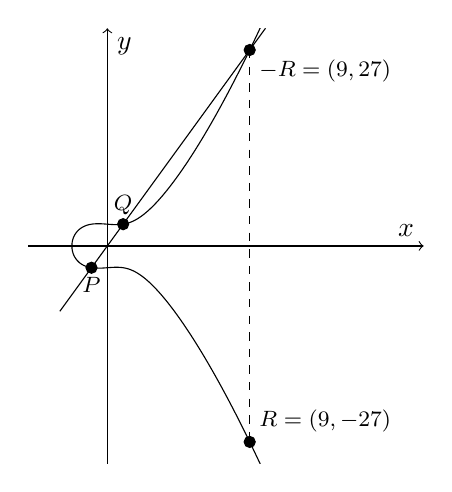
\begin{tikzpicture}

\begin{axis}[%
width=2.6in,
height=2.8in,
axis lines=middle,
axis line style={->},
tick style={color=black},
xtick=\empty,ytick=\empty,
xlabel=$x$,
ylabel=$y$,
xmin=-5,
xmax=20,
ymin=-30,
ymax=30
]

\addplot[
domain=-3:10, 
samples=100] {
3 * x
};

\addplot [forget plot]
  table[row sep=crcr]{%
-2.25	0\\
-2.24	0.023999999999938\\
-2.23	0.374743912558965\\
-2.22	0.528159066948584\\
-2.21	0.645088366039879\\
-2.2	0.742967024840266\\
-2.19	0.828577697020623\\
-2.18	0.90541040418144\\
-2.17	0.975544463363921\\
-2.16	1.04033840648127\\
-2.15	1.10073838853744\\
-2.14	1.15743509537252\\
-2.13	1.21095127895386\\
-2.12	1.2616940992174\\
-2.11	1.3099881678855\\
-2.1	1.35609734163887\\
-2.09	1.4002396223504\\
-2.08	1.44259765700628\\
-2.07	1.48332632957148\\
-2.06	1.52255837326521\\
-2.05	1.56040860033518\\
-2.04	1.59697714448266\\
-2.03	1.63235198410147\\
-2.02	1.66661093240144\\
-2.01	1.69982322610323\\
-2	1.73205080756888\\
-2	1.73205080756888\\
-1.9	2.01022386813011\\
-1.8	2.22890107452081\\
-1.7	2.40561842360753\\
-1.6	2.55029410068721\\
-1.5	2.66926956300783\\
-1.4	2.7669477768834\\
-1.3	2.84657689163669\\
-1.2	2.91067002595622\\
-1.1	2.96124973617559\\
-1	3\\
-0.9	3.02836589599077\\
-0.8	3.04762202380807\\
-0.7	3.05892137852544\\
-0.6	3.06333151976733\\
-0.5	3.06186217847897\\
-0.4	3.05548686791483\\
-0.3	3.0451600943136\\
-0.2	3.03183112986195\\
-0.0999999999999999	3.01645487285986\\
0	3\\
0.1	2.98345437370844\\
0.2	2.96782748824793\\
0.3	2.95414962383424\\
0.4	2.94346734311764\\
0.5	2.93683503111768\\
0.6	2.93530236943317\\
0.7	2.93989795741281\\
0.8	2.95160973029972\\
0.9	2.97136332345945\\
1	3\\
1.1	3.03825607873991\\
1.2	3.08674585931528\\
1.3	3.14594977709435\\
1.4	3.21620894843603\\
1.5	3.29772648956823\\
1.6	3.39057517244493\\
1.7	3.49471028842163\\
1.8	3.60998614955792\\
1.9	3.73617451412538\\
2	3.87298334620742\\
2.1	4.020074626173\\
2.2	4.17708032003216\\
2.3	4.34361600512752\\
2.4	4.51929197994553\\
2.5	4.70372193055669\\
2.6	4.89652938314476\\
2.7	5.09735225386671\\
2.8	5.3058458326642\\
2.9	5.52168452557732\\
3	5.74456264653803\\
3.1	5.9741945063749\\
3.2	6.21031400172326\\
3.3	6.45267386437592\\
3.4	6.70104469467262\\
3.5	6.95521387162178\\
3.6	7.21498440746756\\
3.7	7.48017379477242\\
3.8	7.75061287899222\\
3.9	8.02614477816093\\
4	8.30662386291807\\
4.1	8.59191480404688\\
4.2	8.88189169040019\\
4.3	9.17643721713389\\
4.4	9.47544194219985\\
4.5	9.77880360780397\\
4.6	10.0864265228078\\
4.7	10.3982210016906\\
4.8	10.7141028555824\\
4.9	11.0339929309385\\
5	11.3578166916005\\
5.1	11.6855038402287\\
5.2	12.0169879753622\\
5.3	12.352206280661\\
5.4	12.6910992431704\\
5.5	13.0336103977371\\
5.6	13.3796860949725\\
5.7	13.729275290415\\
5.8	14.082329352774\\
5.9	14.4388018893536\\
6	14.7986485869487\\
6.1	15.161827066683\\
6.2	15.5282967514148\\
6.3	15.8980187444851\\
6.4	16.2709557187032\\
6.5	16.6470718145865\\
6.6	17.0263325469697\\
6.7	17.4087047191915\\
6.8	17.7941563441485\\
6.9	18.1826565715794\\
7	18.5741756210067\\
7.1	18.9686847198218\\
7.2	19.3661560460511\\
7.3	19.7665626753869\\
7.4	20.1698785321082\\
7.5	20.5760783435523\\
7.6	20.9851375978334\\
7.7	21.397032504532\\
7.8	21.8117399581051\\
7.9	22.2292375037922\\
8	22.6495033058122\\
8.1	23.0725161176669\\
8.2	23.4982552543801\\
8.3	23.9267005665219\\
8.4	24.3578324158781\\
8.5	24.7916316526363\\
8.6	25.2280795939762\\
8.7	25.6671580039552\\
8.8	26.1088490745954\\
8.9	26.5531354080832\\
9	27\\
9.1	27.4494262235115\\
9.2	27.9013978144465\\
9.3	28.3558988572043\\
9.4	28.8129137714324\\
9.5	29.2724272994229\\
9.6	29.7344244941785\\
9.7	30.1988907081038\\
9.8	30.6658115822817\\
9.9	31.1351730362945\\
10	31.6069612585582\\
};
\addplot [forget plot]
  table[row sep=crcr]{%
-2.25	-0\\
-2.24	-0.023999999999938\\
-2.23	-0.374743912558965\\
-2.22	-0.528159066948584\\
-2.21	-0.645088366039879\\
-2.2	-0.742967024840266\\
-2.19	-0.828577697020623\\
-2.18	-0.90541040418144\\
-2.17	-0.975544463363921\\
-2.16	-1.04033840648127\\
-2.15	-1.10073838853744\\
-2.14	-1.15743509537252\\
-2.13	-1.21095127895386\\
-2.12	-1.2616940992174\\
-2.11	-1.3099881678855\\
-2.1	-1.35609734163887\\
-2.09	-1.4002396223504\\
-2.08	-1.44259765700628\\
-2.07	-1.48332632957148\\
-2.06	-1.52255837326521\\
-2.05	-1.56040860033518\\
-2.04	-1.59697714448266\\
-2.03	-1.63235198410147\\
-2.02	-1.66661093240144\\
-2.01	-1.69982322610323\\
-2	-1.73205080756888\\
-2	-1.73205080756888\\
-1.9	-2.01022386813011\\
-1.8	-2.22890107452081\\
-1.7	-2.40561842360753\\
-1.6	-2.55029410068721\\
-1.5	-2.66926956300783\\
-1.4	-2.7669477768834\\
-1.3	-2.84657689163669\\
-1.2	-2.91067002595622\\
-1.1	-2.96124973617559\\
-1	-3\\
-0.9	-3.02836589599077\\
-0.8	-3.04762202380807\\
-0.7	-3.05892137852544\\
-0.6	-3.06333151976733\\
-0.5	-3.06186217847897\\
-0.4	-3.05548686791483\\
-0.3	-3.0451600943136\\
-0.2	-3.03183112986195\\
-0.0999999999999999	-3.01645487285986\\
0	-3\\
0.1	-2.98345437370844\\
0.2	-2.96782748824793\\
0.3	-2.95414962383424\\
0.4	-2.94346734311764\\
0.5	-2.93683503111768\\
0.6	-2.93530236943317\\
0.7	-2.93989795741281\\
0.8	-2.95160973029972\\
0.9	-2.97136332345945\\
1	-3\\
1.1	-3.03825607873991\\
1.2	-3.08674585931528\\
1.3	-3.14594977709435\\
1.4	-3.21620894843603\\
1.5	-3.29772648956823\\
1.6	-3.39057517244493\\
1.7	-3.49471028842163\\
1.8	-3.60998614955792\\
1.9	-3.73617451412538\\
2	-3.87298334620742\\
2.1	-4.020074626173\\
2.2	-4.17708032003216\\
2.3	-4.34361600512752\\
2.4	-4.51929197994553\\
2.5	-4.70372193055669\\
2.6	-4.89652938314476\\
2.7	-5.09735225386671\\
2.8	-5.3058458326642\\
2.9	-5.52168452557732\\
3	-5.74456264653803\\
3.1	-5.9741945063749\\
3.2	-6.21031400172326\\
3.3	-6.45267386437592\\
3.4	-6.70104469467262\\
3.5	-6.95521387162178\\
3.6	-7.21498440746756\\
3.7	-7.48017379477242\\
3.8	-7.75061287899222\\
3.9	-8.02614477816093\\
4	-8.30662386291807\\
4.1	-8.59191480404688\\
4.2	-8.88189169040019\\
4.3	-9.17643721713389\\
4.4	-9.47544194219985\\
4.5	-9.77880360780397\\
4.6	-10.0864265228078\\
4.7	-10.3982210016906\\
4.8	-10.7141028555824\\
4.9	-11.0339929309385\\
5	-11.3578166916005\\
5.1	-11.6855038402287\\
5.2	-12.0169879753622\\
5.3	-12.352206280661\\
5.4	-12.6910992431704\\
5.5	-13.0336103977371\\
5.6	-13.3796860949725\\
5.7	-13.729275290415\\
5.8	-14.082329352774\\
5.9	-14.4388018893536\\
6	-14.7986485869487\\
6.1	-15.161827066683\\
6.2	-15.5282967514148\\
6.3	-15.8980187444851\\
6.4	-16.2709557187032\\
6.5	-16.6470718145865\\
6.6	-17.0263325469697\\
6.7	-17.4087047191915\\
6.8	-17.7941563441485\\
6.9	-18.1826565715794\\
7	-18.5741756210067\\
7.1	-18.9686847198218\\
7.2	-19.3661560460511\\
7.3	-19.7665626753869\\
7.4	-20.1698785321082\\
7.5	-20.5760783435523\\
7.6	-20.9851375978334\\
7.7	-21.397032504532\\
7.8	-21.8117399581051\\
7.9	-22.2292375037922\\
8	-22.6495033058122\\
8.1	-23.0725161176669\\
8.2	-23.4982552543801\\
8.3	-23.9267005665219\\
8.4	-24.3578324158781\\
8.5	-24.7916316526363\\
8.6	-25.2280795939762\\
8.7	-25.6671580039552\\
8.8	-26.1088490745954\\
8.9	-26.5531354080832\\
9	-27\\
9.1	-27.4494262235115\\
9.2	-27.9013978144465\\
9.3	-28.3558988572043\\
9.4	-28.8129137714324\\
9.5	-29.2724272994229\\
9.6	-29.7344244941785\\
9.7	-30.1988907081038\\
9.8	-30.6658115822817\\
9.9	-31.1351730362945\\
10	-31.6069612585582\\
};

\addplot [
only marks
] coordinates {
(-1,-3)
} node [pos=0,anchor=north] {\footnotesize $P$};
    
\addplot [
only marks
] coordinates {
(1,3)
} node [pos=0,anchor=south] {\footnotesize $Q$};

\addplot [
only marks
] coordinates {
(9,27)
} node [pos=0,anchor=north west] {\footnotesize $-R=(9,27)$};

\addplot [
only marks
] coordinates {
(9,-27)
} node [pos=0,anchor=south west] {\footnotesize $R=(9,-27)$};

\addplot[color=black,dashed]
coordinates {
(9,27)
(9,-27)
};
\end{axis}
\end{tikzpicture}%
    \label{fig:15-1-b}
  }
  \caption{实数域上的曲线 $y^2=x^3-x+9$}
  \label{fig:15-1}
\end{figure}

我们将在下一节展示如何加强这个加法规则,使得曲线上的点集能够构成一个群。数论中一些最优雅的结论,以及一些深刻的开放性问题,都来自于试图理解椭圆曲线上的有理点群的特性。

我们再说回丢番图,他在式 \ref{eq:15-1} 上寻找有理点的方法是我们刚才介绍的方法的一个变体。丢番图没有选择过两个不同的点的直线,而是选择了在其中一个已知点上作一条该曲线的切线。假设我们在点 $P=(-1,-3)$ 上作一条曲线的切线。和之前一样,不难证明,在有理系数的三次曲线上,如果 $(x_1,y_1)$ 是一个有理点,且 $y_1\neq0$,那么曲线在 $(x_1,y_1)$ 处的切线一定与曲线相交于另一个点 $T$,且 $T$ 也必然是一个有理点。在我们的例子中,曲线在 $P=(-1,-3)$ 处的切线是 $y=-{1/3}x-{10/3}$,该直线与曲线的另一个交点是 $({19/9},-{109/27})$,该点确实是一个有理点。这种方法被称为\textbf{切线法 (tangent method)},它是在 $y_1\neq0$时从一个给定的有理点 $(x_1,y_1)$ 建立一个新有理点的另一种方法。正如我们将看到的,它相当于将点 $P$ 与自己相加,即计算 $P\boxplus P$。
\section{有限域上的椭圆曲线}\label{sec:15-2}

式 \ref{eq:15-1} 中的曲线是定义在有理数上的椭圆曲线的一个例子。对于密码学应用,我们主要关心有限域上的椭圆曲线。简单起见,我们只考虑定义在有限域 $\mathbb{F}_p$ 上的椭圆曲线,其中 $p>3$ 是一个素数。

\begin{definition}\label{def:15-1}
令 $p>3$ 是一个素数,则定义在 $\mathbb{F}_p$ 上的\textbf{椭圆曲线 (elliptic curve)} $E$ 满足方程:
\begin{equation}\label{eq:15-3}
y^2=x^3+ax+b
\end{equation}
其中 $a,b\in\mathbb{F}_p$ 满足 $4a^3+27b^2\neq0$。我们用 $E/\mathbb{F}_p$ 表示椭圆曲线 $E$ 定义在 $\mathbb{F}_p$ 上。
\end{definition}

条件 $4a^3+27b^2\neq0$ 确保方程 $x^3+ax+b=0$ 不存在重根。这是为了避免曲线退化所必须的。

\begin{snote}[椭圆曲线上的点集。]
令 $E/\mathbb{F}_p$ 是一条椭圆曲线,并令 $e\geq 1$。对于点 $(x_1,y_1)$,其中 $x_1,y_1 \in \mathbb{F}_{p^e}$,如果该点满足式 \ref{eq:15-3} 的曲线方程,我们就称该点\textbf{在椭圆曲线$E$上}。当 $e=1$ 时,我们称点 $(x_1,y_1)$ 定义在基域 $\mathbb{F}_p$ 上。而当 $e>1$ 时,我们称点 $(x_1,y_1)$ 定义在 $\mathbb{F}_p$ 的一个扩展域上。

曲线中还包含一个额外的``特殊"点 $\mathcal{O}$,称为\textbf{无穷远点 (the point at infinity)}。稍后我们就会明白定义该点的意义。我们用 $E(\mathbb{F}_{p^e})$ 表示曲线 $E$ 上所有定义在 $\mathbb{F}_{p^e}$ 上的点的集合,包括点 $\mathcal{O}$。

举个例子,考虑一条定义在 $\mathbb{F}_{11}$ 上的椭圆曲线 $E: y^2=x^3+1$。于是:
\begin{equation}\label{eq:15-4}
E(\mathbb{F}_{11})=\left\{\mathcal{O},\,(-1,0),\,(0,\pm1),\,(9,\pm2),\,(6,\pm3),\,(8,\pm4),\,(3,\pm5)\right\}
\end{equation}
该曲线有 $12$ 个 $\mathbb{F}_{11}$ 上的点,所以我们记 $|E(\mathbb{F}_{11})|=12$。

Hasse 的一个经典结论表明 $|E(\mathbb{F}_{p^e})|=p^e+1-t$,其中 $t$ 是一个区间 $|t|\leq 2\sqrt{p^e}$ 中的整数。这表明 $E(\mathbb{F}_{p^e})$ 上点的数量接近 $p^e+1$。式 \ref{eq:15-4} 中的集合 $E(\mathbb{F}_p)$ 正好有 $p+1$ 个点(因此有 $t=0$)。
\end{snote}

\begin{remark}\label{remark:15-1}
Schoof 的一个优雅的算法可以用于计算 $E(\mathbb{F}_{p^e})$ 中点的数量,其时间复杂度为 $\log(p^e)$ 的一个多项式。因此,即使对于一个很大的素数 $p$,我们也可以有效地计算出 $|E(\mathbb{F}_{p^e})|$。
\end{remark}

\begin{snote}[加法法则。]
正如我们在上一节中所讨论的,存在一个非常自然的定义在椭圆曲线的点集上的群操作法则。该群操作可以使用符号``$\boxplus$"来表示点的加法。我们将无穷远处的点 $\mathcal{O}$ 定义为单位元:对于所有的 $P\in E(\mathbb{F}_{p^e})$,我们定义 $P\boxplus\mathcal{O}=\mathcal{O} \boxplus P=P$。

现在,令 $P=(x_1, y_1)$ 和 $Q=(x_2,y_2)$ 为 $E(\mathbb{F}_{p^e})$ 上的两个点。那么,这两点的和 $P\boxplus Q$ 由以下三条规则之一定义:
\begin{itemize}
	\item 如果 $x_1 \neq x_2$,我们使用割弦法。令 $s_\mathrm{c}:=(y_1-y_2)/(x_1-x_2)$ 为经过点 $P$ 和点 $Q$ 的直线的斜率。定义:
		\[
			x_3:=s_\mathrm{c}^2-x_1-x_2
			\quad\text{and}\quad
			y_3:=s_\mathrm{c}(x_1-x_3)-y_1
		\]
	\item 如果 $x_1=x_2$ 且 $y_1=y_2$(即 $P=Q$),但 $y_1 \neq0$,我们使用切线法。令 $s_\mathrm{t}:=(3x_1^2+a)/(2y_1)$ 为曲线在点 $P$ 处的切线的斜率。定义:
		\[
			x_3:=s_\mathrm{t}^2-2x_1
			\quad\text{and}\quad
			y_3:=s_\mathrm{t}(x_1-x_3)-y_1
		\]
	\item 如果 $x_1=x_2$ 且 $y_1=-y_2$,则定义 $P\boxplus Q:=\mathcal{O}$。
\end{itemize}
这个加法法则保证 $E(\mathbb{F}_{p^e})$ 必然是一个群,且该群的单位元就是无穷远点。每个点 $\mathcal{O}\neq P=(x_1,y_1)\in E(\mathbb{F}_{p^e})$ 都有一个加法逆元,即 $-P=(x_1,-y_1)$。最后,我们可以证明,这个加法法则具有结合性。群上的操作显然是可交换的,对于所有的 $P,Q \in E(\mathbb{F}_{p^e})$,我们都有 $P\boxplus Q=Q\boxplus P$,所以该群也必然是一个阿贝尔群。

就像其他群中那样,对于一个点 $P\in E(\mathbb{F}_{p^e})$,我们记 $2P:=P\boxplus P$,$3P:=P\boxplus P\boxplus P$,以此类推。更一般地,对于任意正整数 $\alpha$,我们都有 $\alpha P = (\alpha - 1)P \boxplus P$。注意到,使用平方求幂算法(见附录 \ref{chap:A}),$\alpha P$ 的计算可以用最多 $2\log_2\alpha$ 次群操作完成。
\end{snote}

\subsection{Montgomery 曲线和 Edwards 曲线}

式 \ref{eq:15-3} 中的椭圆曲线方程被称为曲线的 \textbf{Weierstrass 形式}。还有有许多等价的描述椭圆曲线的方法,有些比 Weierstrass 形式更适合计算。我们下面举两个例子。

\begin{snote}[Montgomery 曲线。]
用变量 $u$ 和 $v$ 表示的 \textbf{Montgomery 曲线} $E/\mathbb{F}_p$ 可以被写为:
\[
Bv^2=u^3+Au^2+u
\]
其中 $A,B\in\mathbb{F}_p$,且 $B(A^2-4)\neq0$。令 $u=Bx-{A/3}$ 和 $v=By$,我们就可以将该曲线方程改写为 Weierstrass 形式。Montgomery 曲线上的点的数量 $|E(\mathbb{F}_{p^e})|$ 总是能被 $4$ 整除。练习 \ref{exer:15-4} 探讨了 Montgomery 曲线在计算上的优势。它们也会在下一节中出现。

一些定义在 $\mathbb{F}_p$ 上的 Weierstrass 曲线不能通过变量代换被转换成 $\mathbb{F}_p$ 上的 Montgomery 曲线。比如说,如果 Weierstrass 曲线在 $\mathbb{F}_p$ 上有奇数个点,那么它在 $\mathbb{F}_p$ 上就没有 Montgomery 形式。这样的 Weierstrass 曲线就无法受益于 Montgomery 曲线带来的速度提升了。下一节中将要讨论的曲线 P256 就是一个这样的曲线的例子。
\end{snote}

\begin{snote}[Edwards 曲线。]
另一种描述椭圆曲线 $E/\mathbb{F}_p$ 的途径是 Edwards 形式,它形如:
\[
x^2+y^2=1+dx^2y^2
\]
其中 $d\in\mathbb{F}_p$ 满足 $d\neq0,1$。同样地,这条曲线可以通过一个简单的变量代换转换成 Weierstrass 形式。Edwards 形式的优雅之处在于,弦和切线的加法法则非常容易描述。对于 $E(\mathbb{F}_{p^e})$ 中的点 $P=(x_1,y_1)$ 和 $Q=(x_2,y_2)$,我们定义:
\[
P\boxplus Q=\left(\frac{x_1y_2+x_2y_1}{1+dx_1x_2y_1y_2},\;\frac{y_1y_2-x_1x_2}{1-dx_1x_2y_1y_2}\right)
\]
这就足够了。现在,我们不再需要三条单独的规则了。在这个形式下,单位元是点 $\mathcal{O}=(0,1)$,而点 $(x_1,y_1)$ 的逆元是 $(-x_1,y_1)$。点 $(\pm 1,0)$ 的阶数为 $4$,这意味着 Edwards 曲线上点的个数 $|E(\mathbb{F}_{p^e})|$ 总是能被 $4$ 整除。

Edwards 曲线上加法法则的简单性使得它更容易抵御 \ref{sec:17-6} 节中介绍的计时攻击。同时,这也使得它拥有更加快速的实现。
\end{snote}
\section{椭圆曲线密码学}\label{sec:15-3}

令 $E/\mathbb{F}_p$ 是一条椭圆曲线,并令 $E(\mathbb{F}_{p^e})$ 表示该曲线上的点群。现在,我们有了一个有限群,我们就可以考察这个群上的离散对数、计算性 Diffie-Hellman (CDH) 和确定性 Diffie-Hellman (CDH) 等问题的复杂性。

令 $P$ 是 $E(\mathbb{F}_{p^e})$ 上的一个点,且后者的阶为素数 $q$,则 $qP=\mathcal{O}$。那么,$E(\mathbb{F}_{p^e})$ 上的离散对数问题就是给定一对点 $P$ 和 $\alpha P$ 作为输入,计算 $\mathbb{Z}_q$ 中的一个随机值 $\alpha$ 的问题。正如本章开始时所讨论的那样,对于大多数椭圆曲线来说,针对这个问题的最优已知算法也需要 $\Omega(\sqrt{q})$ 级别的时间。然而,也存在少数几种例外情况,在这些情况下,离散对数的计算要容易得多。下面是两个例子:
\begin{itemize}
	\item 当 $|E(\mathbb{F}_p)|=p$ 时,$E(\mathbb{F}_p)$ 上的离散对数问题可以在多项式时间内解出。
	\item 假设有一个小整数 $\tau>0$ 能使得 $|E(\mathbb{F}_p)|$ 整除 $p^{\tau}-1$。则 $E(\mathbb{F}_p)$ 上的离散对数问题就可以归约到有限域 $\mathbb{F}_{p^\tau}$ 上的离散对数问题,如 \ref{sec:15-4} 节将要介绍的。$\mathbb{F}_{p^\tau}$ 上的离散对数问题可以使用普通数域筛选法 (GNFS) 的离散对数算法变体解决。例如,如果 $\tau$ 很小,比如说 $\tau=2$,并且 $p$ 是一个 $256$ 比特的素数,那么 $E(\mathbb{F}_p)$ 上的离散对数问题就可以被有效地解决:首先,将给定的离散对数问题归约到 $\mathbb{F}_{p^2}$ 上,然后在 $\mathbb{F}_{p^2}$ 上应用 GNFS。因此,这迫使我们确保 $p^\tau$ 足够大,以至于使得 $\mathbb{F}_{p^\tau}$ 上的 GNFS 是完全不可行的。
\end{itemize}
为了避免这些隐患,许多实现都使用固定的曲线集。人们通常认为,这种做法比随机选取一个素数$p$,然后在 $\mathbb{F}_{p}$ 上随机生成一条椭圆曲线要更加安全。两种最广泛使用的曲线被称为 P256 和 Curve25519,我们将在下面分别介绍它们。

一旦我们确保了群 $E(\mathbb{F}_{p})$ 上离散对数、CDH 和 DDH 问题的难度,我们就可以用这个群来实例化我们在前面几章中涉及到的所有构造。由此产生的系统就被称为\textbf{椭圆曲线密码学系统 (elliptic curve cryptosystems)}。

\subsection{P256曲线}

1999年,美国国家标准研究所 (NIST) 公布了一份供联邦政府使用的椭圆曲线清单。这些曲线中最流行的是 \textbf{secp256r1},或者简称 \textbf{P256}。所有 TLS 1.3 的实现都需要支持这种曲线以进行 Diffie-Hellman 密钥交换。它是 TLS 标准(见 \ref{sec:21-10} 节)中唯一的强制性曲线。

P256 曲线定义在素数 $p:=2^{256}-2^{224}+2^{192}+2^{96}-1$ 上。$p$ 的特殊结构可以用来提高模 $p$ 算术运算的性能。该曲线具有标准的 Weierstrass 形式 $y^2=x^3-3x+b$,其中的 $b$ 用十六进制表示为:
\[
b:=\texttt{5ac635d8 aa3a93e7 b3ebbd55 769886bc 651d06b0 cc53b0f6 3bce3c3e 27d2604b}
\]
这条曲线上的点的数量是一个素数 $q$。标准还规定了一个可以生成整个群的点 $G$。

因为素数 $p$ 接近 $2^{256}$,所以点的数量 $q$ 也接近 $2^{256}$。于是,如果假设没有任何捷径的话,在这条曲线上计算离散对数大约就需要 $\sqrt{q}$ 次群运算,也就是大约 $2^{128}$ 次。设计意图是,在这条曲线上计算离散对数(以及 CDH 和 DDH)至少应该和破解 AES-128 一样困难。因此,如果 AES-128 能够被用于加密明文数据,则 P256 也可以被用于 Diffie-Hellman 密钥交换、公钥加密和数字签名。

一些高安全性的应用使用 AES-256 来加密明文数据。在这些情况下,我们应该使用具有更高安全参数的椭圆曲线。一个选择是名为 \textbf{secp521r1} 的曲线,其大小约为 $2^{521}$。它定义在 Mersenne 素数 $p=2^{521}-1$ 上。在这条曲线上计算离散对数被认为至少需要进行 $2^{256}$ 次群运算。

\begin{snote}[参数的选择。]
P256 中那个看起来很奇怪的参数 $b$ 是如何被选出来的?答案是,我们并不清楚。该标准列出了一个无法解释的常数,称为\textbf{种子} $S$。这个种子作为输入参数被提供给一个公开的确定性算法中以产生参数 $b$。这个过程被设计为以伪随机方式选择一条能抵御所有已知的离散对数攻击的曲线。

我们并不清楚种子 $S$ 是如何被选出来的。这可能会让想要使用 P256 的外国政府担心。他们可能会忧虑种子是以对抗性的方式选择的,这样,产生种子的组织就可以有效地计算出所产生的曲线的离散对数。但目前我们尚不知道这样的种子是怎么被选出来的,所以这种担心只是一种耐人寻味的猜测。就我们目前所知,P256 仍是一个可以使用的优良曲线,它仍然在实践中被广泛地使用。
\end{snote}

\subsection{Curve25519}

令 $E/\mathbb{F}_p$ 是一条椭圆曲线,并令 $n:=|E(\mathbb{F}_{p})|=p+1-t$。我们将在 \ref{subsec:17-2-4} 小节说明,$E(\mathbb{F}_{p})$ 上的离散对数的计算难度只与 $n$ 的最大素因子相当。具体地说,存在一种离散对数算法,其运行时间为 $\sqrt{q}$,而 $q$ 就是 $n$ 的最大素因子。如果 $n$ 的最大素因子很小,那么 $E(\mathbb{F}_{p})$ 上的离散对数问题也就很简单。出于这个原因,我们始终坚持 $n$ 是一个素数,或者是一个素数的小倍数。我们用 $q$ 来表示 $n$ 的最大素因子。这个 $q$ 也是 $E(\mathbb{F}_{p})$ 的最大素阶子群的大小。

\begin{snote}[扭变安全性。]
每条椭圆曲线 $E/\mathbb{F}_p$ 都有一条与之相关的曲线 $\tilde E/\mathbb{F}_p$,称为 $E$ 的\textbf{扭变 (twist)}。令 $w\in\mathbb{F}_p$ 是 $\mathbb{F}_p$ 中的某个二次非剩余。如果 $E$ 是曲线 $y^2=x^3+ax+b$,那么它的扭变 $\tilde E$ 就是 $wy^2=x^3+ax+b$。假设 $|E(\mathbb{F}_{p})|$ 是奇数。那么我们可以证明,每个 $x\in\mathbb{F}_p$ 要不是 $E(\mathbb{F}_{p})$ 上点的横坐标,要不就是 $\tilde E(\mathbb{F}_{p})$ 上点的横坐标,但不能同时是。由此可以推断,$\tilde E(\mathbb{F}_{p})$ 上点的数量是 $\tilde n:=p+1+t$。回顾一下,$E/\mathbb{F}_p$ 上点的数量是 $p+1-t$。

如果离散对数在 $E(\mathbb{F}_{p})$ 和 $\tilde E(\mathbb{F}_{p})$ 上都是难以解决的,我们就说曲线 $E/\mathbb{F}_p$ 是\textbf{扭变安全 (twist secure)} 的。要使 $E/\mathbb{F}_p$ 是扭变安全的,我们至少需要 $n=|E(\mathbb{F}_{p})|$ 和 $\tilde n= |\tilde E(\mathbb{F}_{p})|$ 都是素数,或者都是大素数的小倍数。

为什么我们需要扭变安全性?考虑这样的一个系统,其中 Bob 有一个私钥 $α\in\mathbb{Z}_q$。在正常的操作下,任何人都可以向 Bob 发送一个点 $P\in E(\mathbb{F}_{p})$,而 Bob 会以点 $\alpha P$ 作为应答。\ref{subsec:11-7-3} 小节中的不经意 PRF 就是这样的一个系统。在应答之前,Bob 最好检查给定的点 $P$ 是否在 $E(\mathbb{F}_{p})$ 上;否则,Bob 发回的应答可能会泄露他的秘钥 $\alpha$,正如练习 15.1 中所讨论的那样(也可以参见备注 12.1,其中出现了一个类似的问题)。检查一个点 $P=(x1,y1)$ 是否满足曲线方程是非常简单和高效的。然而,有些实现采用了练习 15.2 和练习 15.4 中的优化方法,Bob 只会被给予 $P$ 的横坐标,纵坐标既不需要,也不会被发送给他。在这种情况下,检查给定的 $x_1∈\mathbb{F}_p$ 是否有效,就需要对其进行指数运算,以确认 $x^3_1+ax_1+b$ 是否是 $\mathbb{F}_p$ 的二次剩余(见附录 \ref{subsec:a-2-3} 小节)。假设 Bob 跳过这个很耗费资源的检查,那么攻击者就可以向 Bob 发送一个 $x_1∈\mathbb{F}_p$,它是扭变 $\tilde E(\mathbb{F}_{p})$ 上的一个点 $\tilde P$ 的横坐标。然后 Bob 就会应答一个 $\tilde E(\mathbb{F}_{p})$ 上的点 $\alpha\tilde P$ 的横坐标。如果 $\tilde E(\mathbb{F}_{p})$ 上的离散对数是容易的,这个应答就会暴露 Bob 的私钥 $\alpha$。因此,如果 Bob 跳过这个群元素检查,我们必须至少确保 $\tilde E(\mathbb{F}_{p})$ 中的离散对数是难的,这样 $\alpha\tilde P$ 就不会暴露 $\alpha$。扭变安全性正是为了确保这一点。

曲线 P256 的设计并不是扭变安全的。其扭变的大小可以被 $34905=3×5×13×179$ 整除。因此,在扭变上的离散对数比在 P256 上要容易 $\sqrt{34905}\approx187$ 倍(见 \ref{subsec:17-2-4} 小节)。这个事实不容忽视,但是也不应当因此就放弃使用 P256 曲线。
\end{snote}

\begin{snote}[Curve25519。]
Curve25519 的设计能够支持一种优化的群操作,而且是扭变安全的。这条曲线定义在素数 $p:=2^{255}-19$ 上,这就是其名字的由来。这个 $p$ 是小于 $2^{255}$ 的最大素数,这使得 $\mathbb{F}_p$ 上的算术运算速度极快。

将 Curve25519 描述为一条 Montgomery 曲线是非常容易的,即一条形如 $E:By^2=x^3+Ax^2+x$ 的曲线,其中 $A,B\in\mathbb{F}_p$,且 $p>3$。练习 15.4 表明,这种曲线支持一种快速的乘法算法,能够从 $P$ 计算出 $\alpha P$,其中 $P\in E(\mathbb{F}_{p})$,且 $\alpha\in\mathbb{Z}$。我们在前面已经介绍过,一条 Montgomery 曲线上的点的数量 $|E(\mathbb{F}_{p})|$ 总是 $4$ 的倍数。

用 Montgomery 形式描述的 Curve25519 的方程为:
\[
y^2=x^3+486662\cdot x^2+x
\]
这条曲线上的点的数量是一个素数的 $8$ 倍,因此,我们称该曲线的\textbf{协因子 (cofactor)} 为 $8$。该曲线由一个点 $P=(x_1,y_1)$ 生成,其中 $x_1=9$。完整起见,我们注意到,Curve25519 也可以表示为一条 Edwards 曲线 $x^2+y^2=1+(121665/121666)x^2y^2$。
\end{snote}

\begin{snote}[为什么常数是 486662?]
在定义一条 Montgomery 曲线时,$A$ 越小,群运算就越快,正如我们将在练习 15.4 中说明的。为了获得最佳性能,我们需要让 ${(A-2)}/{4}$ 尽量小。设计这条曲线的 Dan Bernstein 选择了尽可能小的 $A$,这样曲线就能安全地抵御已知的离散对数攻击。他还确保该曲线与其扭变的阶都是某个素数的 $4$ 倍或 $8$ 倍。Bernstein 表示:
\begin{quote}
$A$ 的最小正整数选择有 $358990$、$464586$ 和 $486662$。我没有使用 $A=358990$,因为它的一个素因子比 $2^{252}$ 略小,这就导致了一个问题,即标准和实现应该如何处理用户的私钥与该素数相匹配的理论上的可能性;讨论这个问题比换一个 $A$ 还要困难。我不使用 $464586$ 的原因也是如此。因此最后,我选择了 $A=486662$。
\end{quote}
这个说明比 P256 中的那个缺乏解释的常数更能令人信服。
\end{snote}
\section{基于配对的密码学}\label{sec:15-4}

到目前为止,我们将椭圆曲线作为一个有效的群,它上面的离散对数问题以及其变体 CDH 和 DDH 问题都被认为是困难的。这种群能够让我们有效地实例化前面章节中所介绍的许多方案。我们现在声称,某些特定的椭圆曲线拥有一种额外的结构,称为\textbf{配对 (Paring)}。这种结构开创了一个全新的密码学世界,如果没有这种特殊的结构,许多来自离散对数群的方案都无从谈起。由此产生的方案构成了一个全新的领域,称为\textbf{基于配对的密码学 (pairing based cryptography)}。

为了介绍基于配对的方案,我们将把重点放在配对带来的新功能上,并抽象出椭圆曲线群的细枝末节。同前几章一样,我们把群操作用乘法形式表示。注意,这与本章的前几节不同。此前,为了与传统的椭圆曲线密码学的数学符号保持一致,我们一直在使用加法形式表示群操作。

\begin{definition}\label{def:15-2}
令 $\mathbb{G}_0,\mathbb{G}_1,\mathbb{G}_T$ 是三个 $q$ 阶循环群,其中 $q$ 为素数,$g_0\in\mathbb{G}_0$ 和 $g_1\in\mathbb{G}_1$ 是生成元。一个\textbf{配对 (pairing)}是满足以下性质的一个可有效计算函数 $e:\mathbb{G}_0\times\mathbb{G}_1\to\mathbb{G}_T$:
\begin{enumerate}
	\item 双线性 (bilinear):对于所有的 $u,u'\in\mathbb{G}_0$ 和 $v,v'\in\mathbb{G}_1$,我们有:
	\[
		e(u\cdot u',\,v)=e(u,v)\cdot e(u',v)
		\quad\text{and}\quad
		e(u,\,v\cdot v')=e(u,v)\cdot e(u,v')
	\]
	\item 非退化性 (non-degenerate):$g_T:=e(g_0,g_1)$ 是 $\mathbb{G}_T$ 的一个生成元。
\end{enumerate}
当 $\mathbb{G}_0=\mathbb{G}_1$ 时,我们称该配对为一个\textbf{对称配对 (symmetric pairing)}。我们将 $\mathbb{G}_0$ 和 $\mathbb{G}_1$ 称为\textbf{配对群 (pairing groups)} 或原群 (source groups),将 $\mathbb{G}_T$ 称为\textbf{目标群 (target group)}。
\end{definition}

双线性意味着配对有下面将要介绍的核心属性可以应用于所有的结构:对于任意 $\alpha,\beta \in \mathbb{Z}_q$,有:

$$
e(g_0^\alpha,g_1^\beta)=e(g_0,g_1)^{\alpha,\beta}=e(g_0^\beta,g_1^\alpha)
$$

上述等式从下面的等式中得出:

$$
e(g_0^\alpha,g_1^\beta)=e(g_0,g_1^\beta)^{\alpha}=e(g_0^\alpha,g_1)^\beta
$$

而该等式本身就是双线性的直接结果。我们可以注意到,在 $\mathbb{G}_0$ 和 $\mathbb{G}_1$ 这样的循环群中,上述两个等式也等价于配对的双线性性质。

而配对的另一个非退化性保证了配对 $e$ 对于所有输入并不总是输出 $1 \in \mathbb{G}_T$。事实上,我们总是希望离散对数问题在群 $\mathbb{G}_0$ 和 $\mathbb{G}_1$ 上尽量困难,而很多构造还要求其他的一些问题是困难的,比如 CDH 和 DDH 的某些变体。

直接结果

视 $\mathbb{G}_0$ 和 $\mathbb{G}_1$ 的性质,配对 $e:\mathbb{G}_0 \times \mathbb{G}_1 \to \mathbb{G}_T$ 也会有一些后果。首先,当 $\mathbb{G}_0=\mathbb{G}_1$ 时,可以证明 $\mathbb{G}_0$ 上的 DDH 问题是容易的。想要知道为什么,可以考察三元组 $(u,v,w)=(g_0^\alpha,g_0^\beta,g_0^\gamma)\in\mathbb{G}^3$,我们可以通过验证:

$$
e(u,v)\overset{?}=e(g_0,w)
$$

得到 $\mathbb{Z}_q$ 上的 $\gamma=\alpha\cdot\beta$ 是否成立。根据[式 15.5](https://www.notion.so/aef50a5da9144c7fa4a8ca1c801017e6),我们知道当且仅当:

$$
e(g_0,g_0)^{\alpha\beta}=e(g_0,g_0)^\gamma
$$

时,上述[等式](https://www.notion.so/aef50a5da9144c7fa4a8ca1c801017e6)成立,而该等式当且仅当 $\gamma=\alpha\cdot\beta$ 时成立,此时 $(u,v,w)$ 是一个 DH 三元组。因此 DDH 是容易的。

这意味着乘性 ElGamal 加密方案在对称配对群中会丧失语义安全性,因此不应该被用在这样的群中。同样地,完整 ElGamal 加密方案 $\mathcal{E}_{\rm EG}$ 也不能用基于 DDH 的分析来证明其安全性。然而,$\mathcal{E}_{\rm EG}$ 仍然可以在随机预言机模型中基于 CDH 证明其安全性。

对于非对称配对,即 $\mathbb{G}_0\neq\mathbb{G}_1$ 的情况,DDH 假设在 $\mathbb{G}_0$ 和 $\mathbb{G}_1$ 中都仍然有可能成立。事实上,对于大多数基于椭圆曲线的非对称配对,DDH 假设被认为在 $\mathbb{G}_0$ 和 $\mathbb{G}_1$ 上仍然成立。

其次,在 $\mathbb{G}_0$ 或 $\mathbb{G}_1$ 中计算离散对数不会比在目标群 $\mathbb{G}_T$ 中计算离散对数更难。想知道为什么,假设我们有一个 $u_0=g_0^\alpha\in\mathbb{G}_0$,并被要求计算其离散对数 $\alpha\in\mathbb{Z}_q$。为此,我们计算 $u=e(u_0,g_1)$ 并令 $g_T=e(g_0,g_1)$。可以观察到 $u\in\mathbb{G}_T$ 满足 $u=(g_T)^\alpha$,因此我们可以通过计算以 $g_T$ 为基底的 $u$ 的离散对数来找到 $\alpha$。因此,如果 $\mathbb{G}_T$ 中的离散对数问题很容易,那么 $\mathbb{G}_0$ 中的离散对数问题也很容易。类似的论证也适用于 $\mathbb{G}_1$。因此,为了使离散对数在 $\mathbb{G}_0$ 和 $\mathbb{G}_1$ 中都是困难的,我们必须谨慎选择群,使得目标群 $\mathbb{G}_T$ 中的离散对数也是困难的。

基于椭圆曲线构建配对

一个配对 $e:\mathbb{G}_0 \times \mathbb{G}_1 \to \mathbb{G}_T$ 通常是由椭圆曲线 $E/\mathbb{F}_p$ 构造出来的。来自椭圆曲线的最自然和有效的配对是不对称的,即 $\mathbb{G}_0\neq\mathbb{G}_1$。出于这个原因,我们将使用非对称配对来描述本章中的所有基于配对的系统。

一个由椭圆曲线 $E/\mathbb{F}_p$ 构造的配对 $e:\mathbb{G}_0 \times \mathbb{G}_1 \to \mathbb{G}_T$ 中的群 $\mathbb{G}_0$,$\mathbb{G}_1$ 和 $\mathbb{G}_T$ 具有以下特性:

- $\mathbb{G}_0$ 是 $E(\mathbb{F}_{p})$ 的一个 $q$ 阶子群,其中 $q$ 为素数;
- $\mathbb{G}_1$ 是 $E(\mathbb{F}_{p^d})$ 的一个 $q$ 阶子群,其中 $d>0$ 且 $\mathbb{G}_1\cap\mathbb{G}_0=\{\mathcal{O}\}$;
- $\mathbb{G}_T$ 是有限域 $\mathbb{F}_{p^d}$ 的一个 $q$ 阶乘法子群。

整数 $d>0$ 被称为曲线的**嵌入度 (embedding degree)**。显然 $d$ 需要小一些以便 $\mathbb{G}_1$ 和 $\mathbb{G}_T$ 中的元素能有效表示。如果 $d$ 很大,我们就无法写下 $\mathbb{G}_1$ 和 $\mathbb{G}_T$ 中的元素。$d$ 相对小的椭圆曲线,比如 $d≤16$ 的曲线,被称为**配对友好的椭圆曲线 (pairing friendly elliptic curve)**。

因为 $\mathbb{G}_0$ 定义在基域 $\mathbb{F}_p$ 上,而 $\mathbb{G}_1$ 定义在更大的域 $\mathbb{F}_{p^d}$ 上,所以 $\mathbb{G}_0$ 中的元素通常比 $\mathbb{G}_1$ 中的元素短得多。这在选择每个群所扮演的角色时起到重要的作用。例如为了最大限度地减少密文的长度,我们将倾向于把密文中出现的群元素放在 $\mathbb{G}_0$ 中。

椭圆曲线上的配对函数 $e$ 来自于一个叫做 **Weil 配对**的代数配对。这种配对可以用维克多-米勒算法有效计算。在实践中我们通常使用 Weil 配对的变种,称为 Tate 和 Ate 配对,维克多-米勒算法对于这些配对更加有效。

实践中最常用的曲线被称为 bn256 和 bls381。这两条曲线的嵌入度 $d=12$,群阶 $q$ 是 256 位素数。两条曲线都定义在素数域上:bn256 定义在一个 256 比特的素数域,bls381 定义在一个 381 比特的素数域。曲线 bls381 被认为提供了更好的安全性,因为 $\mathbb{G}_T$ 中的离散对数更难,但 bls381 中的算术由于素数更大而更慢。

配对的性能

令 $e:\mathbb{G}_0 \times \mathbb{G}_1 \to \mathbb{G}_T$ 是一个由配对友好的椭圆曲线 $E/\mathbb{F}_p$ 构造出来的配对,群 $\mathbb{G}_0$,$\mathbb{G}_1$ 和 $\mathbb{G}_T$ 的阶都为素数 $q$。计算配对需要进行 $O(\log q)$ 次 $\mathbb{F}_p$ 上的算术运算,这类似于在 $\mathbb{G}_0$ 和 $\mathbb{G}_1$ 上的指数运算。然而在实践中,计算配对所需的时间往往比指数运算更长,因此我们希望在设计中尽量减少配对的计算复杂度。为了了解相对的计算开支,下面的表格展示了在曲线 bn256 上进行指数和配对运算的时间复杂度。可以看出,$\mathbb{G}_0$ 中的配对运算比指数运算慢 10 倍左右。

![Benchmarks for pairings on the curve bn256](https://s3-us-west-2.amazonaws.com/secure.notion-static.com/3e5dfb04-6ee7-4232-a02c-c60a0fc8fe94/Untitled.png)

Benchmarks for pairings on the curve bn256

在实现配对时,可以进行许多优化:

- 首先,当配对的其中一个输入是固定的时,就有可能通过预处理大大加快配对的计算速度。具体来说,假设人们需要计算许多配对 $e(u,v_i)$,其中 $i=1,2,\dots,n$,$u\in\mathbb{G}_0$ 是固定的。那么就有可能建立一个只取决于 $u$ 的表。一旦构建了这个表,计算每个配对就比没有预处理的情况快得多。
- 其次,配对乘积 $\prod_{i=1}^ne(u_i,v_i)$ 的计算速度可以比逐个计算 $n$ 个配对还要快。例如,配对计算的最后一步是将计算值进行一个固定级数的幂运算。这个最后的指数化可以在乘积的所有配对中汇总,对整个乘积只做一次。

通常,把这两种优化结合在一起会带来显著的速度提升。
\section{来自配对的签名方案}\label{sec:15-5}

配对使得许多新的高级加密和签名方案,以及其他密码学原语成为可能。在这一节中,我们将介绍几种基于配对的新签名方案,它们具备非常有趣的特性。

在 \ref{subsec:15-5-1} 小节,我们会介绍 \emph{BLS 签名方案}。BLS 签名的一个很好的特征是紧凑性——一个签名就是一个单一且简短的群元素。该方案的另一个优异的特性是支持\emph{签名聚合},这是一种可以将许多签名公开地压缩成一个单一且简短的\emph{聚合}签名的方法。这是一个我们以前从未见过的签名方案的新功能。我们将在 \ref{subsec:15-5-2} 和 \ref{subsec:15-5-3} 两个小节讨论这一问题。最后,在 \ref{subsec:15-5-4} 小节中,我们还会提出两个基于配对的签名方案,它们都可以被证明是安全的,而且不依赖于随机预言机模型。请注意,除了第\ref{chap:14}章(特别是 \ref{sec:14-6} 节)所介绍的基于哈希的签名方案外,我们到目前为止所看到的所有其他签名方案的安全性都依赖于随机预言机模型。我们将要在 \ref{subsec:15-5-4} 小节介绍的基于配对的方案所产生的签名比基于哈希的方案所产生的签名要短得多。

\subsection{BLS 签名方案}\label{subsec:15-5-1}

令 $e:\mathbb{G}_0\times\mathbb{G}_1\to\mathbb{G}_\mathrm{T}$ 是一个配对,其中 $\mathbb{G}_0,\mathbb{G}_1,\mathbb{G}_\mathrm{T}$ 是三个 $q$ 阶循环群,$q$ 为素数,并且 $g_0\in\mathbb{G}_0$ 和 $g_1\in\mathbb{G}_1$ 是生成元。此外,我们还需要一个能将有限集 $\mathcal{M}$ 中的消息映射为 $\mathbb{G}_0$ 中元素的哈希函数 $H$。

BLS 签名方案,表示为 $\mathcal{S}_{\rm BLS}=(G,S,V)$,有消息空间 $\mathcal{M}$,工作流程如下:
\begin{itemize}
	\item $G()$:密钥生成算法运行如下:
	\[
		\alpha\stackrel{R}\leftarrow\mathbb{Z}_q,\quad
    	u\leftarrow g_1^\alpha \in \mathbb{G}_1
	\]
	公钥为 $pk:=u$,私钥为 $sk:=\alpha$。
	\item $S(sk,m)$:为了使用私钥 $sk=\alpha\in\mathbb{Z}_q$ 对消息 $m\in\mathcal{M}$ 进行签名,进行如下操作:
	\[
		\sigma\leftarrow H(m)^\alpha\in\mathbb{G}_0
	\]
	输出 $\sigma$。
	\item $V(pk,m,\sigma)$:为了验证消息 $m\in\mathcal{M}$ 上的签名 $\sigma\in\mathbb{G}_0$,使用公钥 $pk=u\in\mathbb{G}_1$,当:
	\[
		e\big(H(m),\,u\big)=e(\sigma,g_1)
	\]
	时,输出 $\mathsf{accept}$。
\end{itemize}

很容易验证,有效消息总是能被接受:对于所有的公钥 $u\leftarrow g_1^\alpha$ 和消息 $m\in\mathcal{M}$,合法签名 $\sigma \leftarrow H(m)^\alpha$  将会被验证者接受,因为:
\[
e\big(H(m),\,u\big)=e\big(H(m),\,g_1^\alpha\big)=e\big(H(m)^\alpha,\,g_1\big)=e(\sigma,\,g_1)
\]

如上所述,签名落在群 $\mathbb{G}_0$ 上,而公钥则在群 $\mathbb{G}_1$ 上。我们在上一节中提到,$\mathbb{G}_0$ 上的元素与 $\mathbb{G}_1$ 上的元素相比有更短的表示。因此,正如所述的,这个签名方案是为短签名而特别优化的——一个签名就是 $\mathbb{G}_0$ 上的一个元素。我们同样可以通过定义一个对称方案来为短公钥的需求进行优化,只要将 $\mathbb{G}_0$ 和 $\mathbb{G}_1$ 的角色对调即可:此时签名在群 $\mathbb{G}_1$ 上,而公钥在群 $\mathbb{G}_0$ 上。下面的安全分析同样适用于这种对称方案。

\begin{snote}[唯一签名。]
$\mathcal{S}_{\rm BLS}$ 方案是一个\textbf{唯一签名方案 (unique signature scheme)}:对于一个给定的公钥,每条消息 $m\in\mathcal{M}$ 都只有\emph{唯一的}签名 $\sigma\in\mathbb{G}_0$ 能够被验证算法接受为 $m$ 的有效签名。这意味着,如果 $\mathcal{S}_{\rm BLS}$ 是安全的,那么在定义 \ref{def:13-3} 的意义上,它也一定是强安全的。
\end{snote}

\begin{snote}[安全性。]
我们可以证明,当 $H:\mathcal{M}\to\mathbb{G}_0$ 被建模为一个随机预言机时,$\mathcal{S}_{\rm BLS}$ 是安全的。我们需要对 CDH 假设做一个微小的改动,使得标准 CDH 假设能够适用于两个群的情况。
\end{snote}

\begin{game}[co-CDH]\label{game:15-1}
对于一个给定对手 $\mathcal{A}$,攻击游戏按照如下方式进行:
\begin{itemize}
	\item 挑战者计算:
	\[
		\alpha,\beta \overset{\rm R}\leftarrow \mathbb{Z}_q,\quad
    	u_0 \leftarrow g_0^\alpha,\quad
    	u_1 \leftarrow g_1^\alpha,\quad
    	v_0 \leftarrow g_0^\beta,\quad
    	z_0 \leftarrow g_0^{\alpha\beta}
	\]
	并将元组 $(u_0, u_1, v_0)$ 交给对手。注意 $\alpha$ 被使用了两次,一次在 $\mathbb{G}_0$ 上,另一次在 $\mathbb{G}_1$ 上。
	\item 对手输出某个 $\hat{z}_0 \in \mathbb{G}_0$。
\end{itemize}
我们将 $\mathcal{A}$ 解决 $e$ 的 co-CDH 问题的优势表示为 $\mathrm{coCDH}\mathsf{adv}[\mathcal{A},e]$,即 $\hat{z}_0 = z_0$ 成立的概率。
\end{game}

这里我们使用 $z_0$ 表示 Diffie-Hellman 秘密 $z_0:=g_0^{\alpha\beta}$。更一般地,在本章的攻击游戏中,我们总是使用变量 $z$ 来表示对手试图从随机采样中计算或区分出的未知值。

\begin{definition}[co-CDH 假设]\label{def:15-3}
如果对于所有的有效对手 $\mathcal{A}$,$\rm{coCDH\mathsf{adv}}[\mathcal{A},e]$ 的值都可忽略不计,我们就称 \textbf{co-CDH} 假设对配对 $e$ 成立。
\end{definition}

当 $e$ 是一个对称配对时,我们有 $\mathbb{G}_0=\mathbb{G}_1$ 且 $g_0=g_1$,在这种情况下,co-CDH 假设与标准 CDH 假设相同。现在,我们可以证明 $\mathcal{S}_{\rm BLS}$ 的安全性。

\begin{theorem}\label{theo:15-1}
令 $e: \mathbb{G}_0 \times \mathbb{G}_1 \rightarrow \mathbb{G}_\mathrm{T}$ 是一个配对,并令 $H: \mathcal{M} \rightarrow \mathbb{G}_0$ 是一个哈希函数。假设 co-CDH 假设对 $e$ 成立,并且 $H$ 被建模为一个随机预言机,那么派生的 BLS 签名方案 $\mathcal{S}_{\rm BLS}$ 是一个安全的签名方案。
\begin{quote}
特别地,令 $\mathcal{A}$ 是一个在攻击游戏 \ref{game:13-1} 的随机预言机版本中攻击 $\mathcal{S}_{\rm BLS}$ 的有效对手。此外,假设 $\mathcal{A}$ 最多能够发起 $Q_{\rm s}$ 次签名查询。那么存在一个有效 co-CDH 对手 $\mathcal{B}$,其中 $\mathcal{B}$ 是一个围绕 $\mathcal{A}$ 的基本包装器,满足:
\end{quote}
\begin{equation}\label{eq:15-6}
\rm{SIG^{ro}\mathsf{adv}}[\mathcal{A},\mathcal{S}_{BLS}]\leq2.72\cdot(Q_s+1)\cdot\rm{coCDH\mathsf{adv}}[\mathcal{B},e]
\end{equation}
\end{theorem}

\begin{proof}[证明思路]
该定理的证明模仿了 RSA-FDH 签名方案(即定理 \ref{theo:13-4})的安全性证明。对手 $\mathcal{B}$ 被给定一个元组 $(u_0=g_0^\alpha, u_1=g_1^\alpha, v_0=g_0^\beta)$,其中 $\alpha,\beta\overset{\rm R}\leftarrow\mathbb{Z}_q$,就像在 co-CDH 攻击游戏中那样。它需要计算 $z_0:=g_0^{\alpha\beta}=v_0^\alpha$。对手首先向签名伪造者 $\mathcal{A}$ 发送 BLS 公钥 $pk:=u_1$。

接下来,签名伪造者 $\mathcal{A}$ 向 $H$ 发起一连串的签名查询 $Q_{\rm s}$ 和随机预言机查询 $Q_{\rm ro}$。对于 $j=1,2,\dots$,我们的对手 $\mathcal{B}$ 会应答第 $j$ 个随机预言机查询 $H(m_j)$,方法是随机选取 $\rho_j\overset{\rm R}\leftarrow\mathbb{Z}_q$,并置 $H(m_j):=g_0^{\rho_j}$。这使得对手 $\mathcal{B}$ 能够应答所有来自 $\mathcal{A}$ 的签名查询。消息 $m_j$ 上的签名就是 $\sigma_j=u_0^{\rho_j}$,这是因为 $\sigma_j:=H(m_j)^\alpha=g_0^{\rho_j\alpha}=u_0^{\rho_j}$。我们的 $\mathcal{B}$ 就能够利用 co-CDH 挑战中给定的 $u_0$ 来计算 $\sigma_j$。这就是我们在挑战中包含 $u_0$ 的原因。

最后,$\mathcal{A}$ 会输出一个有效的签名伪造 $(m,\sigma)$,其中 $\sigma=H(m)^\alpha$。我们知道,$H(m)$ 要不是在 $\mathcal{A}$ 对 $H(m)$ 发出一个显式的随机预言机查询时确定的,要不就是在 $\mathcal{A}$ 输出最终的签名伪造时定义的(需要注意,$m$ 不能出现在 $\mathcal{A}$ 的签名查询中)。因此,$H(m)$ 是在对 $H$ 的 $Q_{\rm ro}+1$ 次查询中的某一次被确定的。假设 $\mathcal{A}$ 在第 $\nu$ 次哈希查询中对 $H(m)$ 发起查询,其中 $1\leq\nu\leq Q_{ro}+1$。一种证明的策略是在游戏开始时让 $\mathcal{B}$ 尝试猜测 $\nu$。$\mathcal{B}$ 在游戏开始时从 $\{1,\dots,Q_{\rm ro}+1\}$ 中随机选择一个 $\omega$,并对第 $\omega$ 次哈希查询应答 $H(m_\omega):=v_0$。如果 $\mathcal{B}$ 很幸运地选中了正确的 $\omega$,即使得 $\omega=\nu$,那么 $\mathcal{A}$ 输出的 $m=m_\omega$ 的签名 $\sigma$ 就满足 $\sigma=H(m)^\alpha=H(m_\omega)^\alpha=v_0^\alpha=z_0$,这也就是 $\mathcal{B}$ 赢得 co-CDH 游戏所需要的值。

这种计算 $z_0$ 的证明策略的效果很好,但是与 $\mathcal{A}$ 相比,$\mathcal{B}$ 的成功概率会有一个 $Q_{\rm ro}+1$ 系数的损失,这是因为 $\mathcal{B}$ 需要在游戏开始的时候正确猜测出 $\nu$。如式 \ref{eq:15-6} 所述,如果使用用于 RSA 假设的引理 \ref{lemma:13-6} 完全相同的参数,就可以将该损失减少到 $2.72\cdot(Q_{\rm s}+1)$。关于引理 \ref{lemma:13-6} 在 CDH 假设下的类比,可参见练习 \ref{exer:15-5}。练习 \ref{exer:15-5} 表明,本安全证明其实与 \ref{subsec:13-4-2} 小节中的 RSA-FDH 的安全证明完全相同,也给出了式 \ref{eq:15-6} 中的约束。
\end{proof}

\subsection{签名聚合}\label{subsec:15-5-2}

BLS 签名方案是非常灵活的,很容易使用 BLS 建立阈值签名方案(练习 \ref{exer:15-7})或者盲签名方案(练习 \ref{exer:15-6}),甚至可以在多方之间分布式地生成密钥。在本小节中,我们将介绍 BLS 的一个特性,称为签名聚合,这是一个我们之前从未见过的新特性。

\textbf{签名聚合(signature aggregation)} 指将不同消息的签名(可能使用不同的签名密钥)压缩成一个短的聚合签名的能力。这个短的聚合签名可以让验证者相信,所有的输入消息都已经被正确的签署了。

\begin{definition}\label{def:15-4}
聚合签名方案 $\mathcal{S}\mathcal{A}$ 是一种包含两个额外的有效算法 $A$ 和 $\textit{VA}$ 的签名方案:
\begin{itemize}
	\item 一个签名聚合算法 $A(\boldsymbol{pk},\boldsymbol{\sigma})$:接受两个等长向量作为输入,即一个公钥向量 $\boldsymbol{pk}=(pk_1,pk_2,\dots,\allowbreak pk_n)$ 和一个签名向量 $\boldsymbol{\sigma}=(\sigma_1,\sigma_2,\dots,\sigma_n)$。它输出一个聚合签名 $\sigma_{\rm ag}$。
	\item 一个1的聚合验证算法 $\textit{VA}(\boldsymbol{pk},\boldsymbol{m},\sigma_{ag})$:接受两个等长向量作为输入,即一个公钥向量 $\boldsymbol{pk}=(pk_1,pk_2,\dots,pk_n)$,一个消息向量 $\boldsymbol{m}=(m_1, m_2, \dots, m_n)$,和一个聚合签名 $\sigma_{\rm ag}$。它输出 $\mathsf{accept}$ 或者 $\mathsf{reject}$。
	\item 如果对于所有的 $\boldsymbol{pk}=(pk_1,pk_2,\dots, pk_n)$,$\boldsymbol{m}=(m_1, m_2, \dots, m_n)$ 和 $\boldsymbol{\sigma}=(\sigma_1, \sigma_2, \dots, \sigma_n)$,只要 $V(pk_i,m_i,\sigma_i)=\mathsf{accept}$ 对所有的 $i=1,2,\dots,n$ 都成立,就有 $\Pr[\textit{VA}(\boldsymbol{pk},\boldsymbol{m},A(\boldsymbol{pk},\boldsymbol{\sigma}))=\mathsf{accept}]=1$,则该方案是正确的。
\end{itemize}
上述方案中,所有输入向量的长度 $n$ 都小于某个上界参数 $N$。
\end{definition}

算法 $A$ 所输出的聚合签名 $\sigma_{\rm ag}$ 应当是短的。不管聚合了多少个签名,$\sigma_{\rm ag}$ 的长度都应当和单个签名的长度差不多。需要注意的是,任何人都可以使用聚合算法 $A$ 来聚合一组给定的签名。聚合不需要知道签名所用的私钥,也不需要与签名者进行交互。特别地,聚合甚至可以在签名者发出签名之后很长时间后才进行。

签名聚合在很多现实世界的场景中都会出现。例如,在一个包含由多个不同权威机构签发的多个证书的证书链中,我们可以将证书链中的所有签名聚合成一个短的聚合签名。这就缩小了证书链的总长度。另一个例子是分布式系统,在这种系统中,多方会定期签名并发布他们对系统状态的观测结果。这些签名会被记录在一个长期日志中。日志管理器可以将所有签名聚合成一个短的聚合签名,以此来压缩日志。这种效率的提升在区块链系统中尤为重要 \cite{ethereum2019specifications}。

在讨论聚合的安全性之前,我们先简单尝试一下聚合 BLS 签名。回顾一下,该方案使用一个哈希函数 $H:\mathcal{M}\rightarrow\mathbb{G}_0$,BLS 公钥是一个群元素 $pk=g_1^\alpha\in\mathbb{G}_1$,而签名是另一个群元素 $\sigma\in\mathbb{G}_0$。考虑如下的简单聚合算法 $A$,它通过简单计算 $n$ 个签名的乘积来聚合这些签名。更准确地说,该方案的工作原理如下:
\begin{quote}
聚合签名算法 $\mathcal{SA}_{\rm BLS}=(\mathcal{S}_{\rm BLS},A,\textit{VA})$:
\begin{itemize}
	\item $A(\boldsymbol{pk}\in\mathbb{G}_1^n,\;\boldsymbol\sigma\in\mathbb{G}_0^n):=\big\{\sigma_{\rm ag}\leftarrow\sigma_1\cdot\sigma_2\cdots\sigma_n\in\mathbb{G}_0,\;\;\text{输出}\;\sigma_{\rm ag}\in\mathbb{G}_0\big\}$。
	\item $\textit{VA}(\boldsymbol{pk}\in\mathbb{G}_1^n,\;\boldsymbol{m}\in\mathcal{M}^n,\;\sigma_\mathrm{ag})$:当:
	\begin{equation}\label{eq:15-7}
	e(\sigma_{\rm ag},g_1)=e\big(H(m_1),pk_1\big)\,\cdots\,e\big(H(m_n),pk_n\big)
	\end{equation}
	时,接受签名。
\end{itemize}
\end{quote}

为了了解为什么验证算法会接受有效聚合签名 $\sigma_{ag}$,不妨观察:

\[
\begin{aligned}
e(\sigma_{\rm ag},g_1)
& =e(\sigma_1\cdots\sigma_n,g_1)
=\prod_{i=1}^{n}e(\sigma_i,g_1)
=\prod_{i=1}^{n}e\big(H(m_i)^{\alpha_i},g_1\big)\\
& =\prod_{i=1}^{n}e\big(H(m_i),g_1^{\alpha_i}\big)
=\prod_{i=1}^{n}e\big(H(m_i),pk_i\big)
\end{aligned}
\]
因此,式 \ref{eq:15-7} 中的等式成立。

\begin{remark}\label{remark:15-2}
尽管我们将聚合的过程描述成一个一次性的过程,但是 BLS 聚合机制也可以逐步完成。我们可以将一些签名聚合起来得到一个聚合签名,并在之后将更多的签名添加到这个聚合中。此外,给定一个聚合签名 $\sigma_{\rm ag}$ 和已经被聚合到 $\sigma_{\rm ag}$ 中的某个签名 $\sigma$,我们可以从 $\sigma_{\rm ag}$ 中移除 $\sigma$,方法是计算 $\sigma_{\rm ag}'\leftarrow{\sigma_{\rm ag}}/{\sigma}$。
\end{remark}

\begin{remark}\label{remark:15-3}
在某些情况下,我们最终会得到一个聚合签名 $\sigma_{\rm ag}$,它包含了签名 $\sigma$ 的多个副本。例如,假设服务器 $S_1$ 聚合了一些用户的签名,并将聚合签名 $\sigma_{\rm ag}^{(1)}$ 发送给服务器 $S_3$。服务器 $S_2$ 聚合了另一组用户的签名,也将聚合签名 $\sigma_{\rm ag}^{(2)}$ 发送给服务器 $S_3$。服务器 $S_3$ 把两个聚合签名 $\sigma_{\rm ag}^{(1)}$ 和 $\sigma_{\rm ag}^{(2)}$ 再次聚合,得到最终的聚合签名 $\sigma_{\rm ag}\leftarrow\sigma_{\rm ag}^{(1)}\cdot\sigma_{\rm ag}^{(2)}$。如果用户 Alice 把她的签名发送给了 $S_1$ 和 $S_2$,她的签名 $\sigma$ 就会被两次包含在最终的聚合签名 $\sigma_{\rm ag}$ 中。这并不影响性能和安全性,但是,验证者在验证时需要知道每个签名在聚合签名中被包含了多少次,以便使用式 \ref{eq:15-7} 正确地验证签名 $\sigma_{\rm ag}$。
\end{remark}

\begin{remark}[快速验证]\label{remark:15-4}
验证式 \ref{eq:15-7} 中的一个由 $n$ 个签名聚合成的签名需要计算 $n+1$ 次配对。当聚合中的所有签名消息都相同时,即 $m_1=m_2=\cdots=m_n=m$ 时,该过程可以被进一步简化。这种情况通常发生在多方对相同的消息 $m$ 进行签名,并需要把这些签名聚合到一个签名 $\sigma_{\rm ag}$ 中的时候。在这种情况下,验证聚合签名 $\sigma_{\rm ag}$ 的式 \ref{eq:15-7} 可以被简化为:
\begin{equation}\label{eq:15-8}
e(\sigma_{\rm ag},g_1)\overset{?}=e\big(H(m),\textit{apk}\big),
\quad\text{其中}\quad
\textit{apk}=pk_1\cdots pk_n \in \mathbb{G}_1
\end{equation}
这样,不管 $n$ 有多大,验证者都只需计算两次配对。上式中的 $\textit{apk}$ 被称为\textbf{聚合公钥 (aggregated public key)}。如果聚合中的签名者都已经在事先固定好,那么这个短的 $\textit{apk}$ 也可以被预先计算,这样,验证者就不再需要存储公钥 $pk_1,\dots,pk_n$ 了。
\end{remark}

\begin{snote}[流氓公钥攻击。]
尽管 BLS 聚合方案 $\mathcal{SA}_{\rm BLS}$ 能够正常工作,但它是完全不安全的。为了解释针对它的攻击,考虑一个用户 Bob,它的公钥是 $pk_{\rm B}:=u_{\rm B}\in\mathbb{G}_1$。对手想要让其他人觉得 Bob 签署了某条消息 $m\in\mathcal{M}$,但 Bob 其实并没有签署它。为此,对手随机选择一个 $\alpha\overset{\rm R}\leftarrow\mathbb{Z}_q$,并计算:
\begin{equation}\label{eq:15-9}
u\leftarrow g_1^\alpha,
\quad
pk_{\rm adv}\leftarrow{u}/{u_{\rm B}}\in\mathbb{G}_1
\end{equation}
公钥 $pk_{\rm adv}$ 对应的私钥是 $\alpha_{\rm adv}:=\alpha-\alpha_{\rm B}$,其中 $\alpha_{\rm B}$ 是 Bob 的私钥。对手并不知道这个私钥,但他仍然可以宣称 $pk_{\rm adv}$ 是它的公钥。我们称这个 $pk_{\rm adv}$ 是一个\textbf{流氓公钥 (rouge public key)}。

公钥 $pk_{\rm B}$ 和 $pk_{\rm adv}$ 的聚合公钥是 $\textit{apk}:=pk_{\rm B}\cdot pk_{\rm adv} = u_{\rm B}\cdot({u}/{u_{\rm B}})=u=g_1^\alpha$,并且对手已经知道了 $\alpha \in \mathbb{Z}_q$。因此,它能够计算出 $\sigma_{\rm ag}:=H(m)^\alpha \in \mathbb{G}_0$。这个 $\sigma_{\rm ag}$ 是使用公钥 $pk_{\rm B}$ 和 $pk_{\rm adv}$ 对消息 $m$ 发出的有效签名。事实上,$\sigma_{\rm ag}$ 总是能够通过式 \ref{eq:15-8} 的验证:
\[
e(\sigma_{\rm ag},g_1)
=e\big(H(m)^\alpha,g_1\big)
=e\big(H(m),g_1^\alpha\big)
=e\big(H(m),u\big)
=e\big(H(m),\textit{apk}\big)
\]
这样,对手就创建了一个聚合签名 $\sigma_{\rm ag}$,使它看起来就好像 Bob 签署了 $m$ 一样。这就完全破坏了聚合签名方案。
\end{snote}

\begin{snote}[安全聚合的定义。]
我们的安全性定义必须正确地建模上述的流氓公钥攻击。在安全游戏中,对手被要求在一系列公钥上创造一个有效的聚合签名,其中,对手能够控制除某一个公钥之外的所有其他公钥。在输出伪造聚合之前,对手可以对不受它控制的那个公钥发起签名查询。
\end{snote}

\begin{game}[聚合签名的安全性]\label{game:15-2}
对于一个给定的聚合签名方案 $\mathcal{SA}=(G,S,V,A,\textit{VA})$(消息空间为 $\mathcal{M}$)以及一个给定对手 $\mathcal{A}$,攻击游戏运行如下:
\begin{quote}
\begin{itemize}
	\item 挑战者计算 $(pk,sk)\overset{\rm R}\leftarrow G()$,并将 $pk$ 发送给 $\mathcal{A}$。
	\item $\mathcal{A}$ 向挑战者发起查询。对于 $i=1,2,\dots$,第 $i$ 个\emph{签名查询}是一条消息 $m^{(i)}\in\mathcal{M}$。挑战者计算 $\sigma_{i}\overset{\rm R}\leftarrow S(sk,m^{(i)})$,然后将 $\sigma_i$ 发送给 $\mathcal{A}$。
	\item 最终,$\mathcal{A}$ 输出一个候选的聚合伪造 $(\boldsymbol{pk},\boldsymbol{m},\sigma_{\rm ag})$,其中 $\boldsymbol{pk}=(pk_1, pk_2, \dots, pk_n)$,$\boldsymbol{m}=(m_1,m_2,\dots,m_n)\in\mathcal{M}^n$。
\end{itemize}
\end{quote}
当下列条件成立时,我们就说对手赢得了这场攻击游戏:
\begin{itemize}
	\item $\textit{VA}(\boldsymbol{pk},\boldsymbol{m},\sigma_{\rm ag})=\mathsf{accept}$,
	\item 至少存在一个 $1\leq j\leq n$ 使得 (1) $pk_j=pk$,并且 (2) $\mathcal{A}$ 未对消息 $m_j$ 发起过签名查询,即 $m_j\notin\{m^{(1)},m^{(2)},\dots\}$。
\end{itemize}
我们将 $\mathcal{A}$ 就 $\mathcal{SA}$ 的优势定义为 $\mathrm{ASIG}\mathsf{adv}[\mathcal{A},\mathcal{SA}]$,其值为 $\mathcal{A}$ 赢得该游戏的概率。
\end{game}

\begin{definition}\label{def:15-5}
如果对于所有的有效对手 $\mathcal{A}$,$\mathrm{ASIG}\mathsf{adv}[\mathcal{A},\mathcal{SA}]$ 的值都可忽略不计,我们就称聚合签名方案 $\mathcal{SA}$ 是安全的。
\end{definition}


\subsection{安全的 BLS 聚合}\label{subsec:15-5-3}

现在我们已经了解了安全性的需求,让我们看看该如何加强式 \ref{eq:15-7} 中的简单聚合流程,来妥善地聚合 BLS 签名。有两种主要方法可以用来防止流氓公钥,它们分别针对不同的使用场景。下面,我们先描述这两种方法,然后证明它们的安全性。

\subsubsection{方法 1:消息增强}\label{subsubsec:15-5-3-1}

想要安全地聚合 BLS 签名,最简单的方法就是把签名公钥添加到每条被签名的消息中。具体来说,修改后的签名方案 $\mathcal{SA}_{BLS}^{(1)}$ 与式 \ref{eq:15-7} 中定义的签名方案 $\mathcal{SA}_{\rm BLS}$ 大致相同,区别在于,现在的签名算法使用一个哈希函数 $H:\mathbb{G}_1\times\mathcal{M}\to\mathbb{G}_0$,并且定义如下:

\vspace*{10pt}

\hspace*{10pt} $S(sk,m):=H(pk,m)^\alpha$,其中 $sk=\alpha \in \mathbb{Z}_q$,$pk \leftarrow g_i^\alpha$。

\vspace*{10pt}

\noindent
被签名的消息实际上是元组 $(pk,m)\in\mathbb{G}_1\times\mathcal{M}$。聚合验证算法也相应地改为对元组 $(pk,m)$ 进行哈希。具体来说,聚合验证算法运行如下:

\vspace*{10pt}

\hspace*{9pt} $\textit{VA}(\boldsymbol{pk}\in\mathbb{G}_1^n,\;\boldsymbol{m}\in\mathcal{M}^n,\;\sigma_{\rm ag})$:\\
\hspace*{70pt} 当 $e(\sigma_{\rm ag},g_1)=e\big(H(pk_1,m_1),pk_1\big)\;\cdots\; e\big(H(pk_n,m_n),pk_n\big)$ 成立时,接受签名。

\vspace*{10pt}

\noindent
我们将在下面的 \ref{subsubsec:15-5-3-3} 小节证明这种方法是安全的。

\subsubsection{方法 2:私钥的持有证明}\label{subsubsec:15-5-3-2}

在方法 $1$ 中,我们将公钥作为每条消息的前缀,其缺点在于,当聚合多个对同一消息的签名时,我们无法再利用备注 \ref{remark:15-4} 中介绍的验证优化方法。在将公钥嵌入消息后,被签名的消息不再是完全相同的,这使得验证者无法再利用式 \ref{eq:15-8} 中的优化验证检验。下面,我们展示另一种聚合方法,它能在事先了解公钥集的情况下利用这种优化。

回顾一下,在式 \ref{eq:15-9} 的流氓公钥攻击中,对手并不知道其流氓公钥 $pk_{\rm adv}$ 所对应的私钥。因此,我们可以要求每个签名者证明自己拥有其公钥所对应的私钥,以此来防止该攻击。

修改后的签名方案 $\mathcal{SA}_{\rm BLS}^{(2)}$ 与式 \ref{eq:15-7} 中定义的签名方案 $\mathcal{SA}_{\rm BLS}$ 大致相同,区别在于,现在密钥生成算法还需要生成一个证明 $\pi$,以证明签名者持有对应的私钥。我们将证明 $\pi$ 附在公钥后,并在聚合验证时一并检查之。特别地,密钥生成和聚合验证算法需要使用一个辅助哈希函数 $H':\mathbb{G}_1\to\mathbb{G}_0$,并且运行如下:
\begin{itemize}
	\item $G():=
	\left\{
	\;
	\begin{aligned}
	& \alpha\overset{\rm R}\leftarrow\mathbb{Z}_q,\quad u\leftarrow g_1^\alpha\in\mathbb{G}_1,\quad\pi\leftarrow H'(u)^\alpha\in\mathbb{G}_0\\
	& \text{输出}\;pk:=(u,\pi)\in\mathbb{G}_1\times\mathbb{G}_0,\quad sk:=\alpha\in\mathbb{Z}_q
	\end{aligned}
	\;
	\right\}
	$
	\item $\textit{VA}(\boldsymbol{pk},\;\boldsymbol{m}\in\mathcal{M}^n,\;\sigma_{\rm ag})$:令 $\boldsymbol{pk}=(pk_1,\dots,pk_n)=\big((u_1,\pi_1),\dots,(u_n,\pi_n)\big)$ 是 $n$ 个公钥,并令 $\boldsymbol{m}=(m_1,m_2,\dots,m_n)$。当:
	\begin{itemize}
		\item 合法证明:对于所有的 $i=1,2,\dots,n$,都有 $e(\pi_i,g_1)=e\big(H'(u_i),u_i\big)$,并且
		\item 合法聚合:$e(\sigma_{\rm ag},g_1)=e\big(H(m_1),u_1\big)\cdots e\big(H(m_n),u_n\big)$。
	\end{itemize}
	时,接受签名。
\end{itemize}

\noindent
公钥中的新项 $\pi=H'(u)^\alpha\in\mathbb{G}_0$ 用于证明公钥的所有者也持有私钥 $\alpha$。这个 $\pi$ 是对公钥 $u\in\mathbb{G}_1$ 的 BLS 签名,但使用的哈希函数是 $H'$ 而不是 $H$。聚合验证算法先会检查给定公钥的所有项 $\pi_1,\pi_2,\dots,\pi_n\in\mathbb{G}_0$ 都是合法的,之后再验证聚合签名 $\sigma_{\rm ag}$ 是否合法,这与 $\mathcal{SA}_{\rm BLS}$ 中完全一致。

我们将在下面的 \ref{subsubsec:15-5-3-3} 小节证明这种方法的安全性。在使用该签名方案时,要点在于,哈希函数 $H'$ 要独立于签署消息的哈希函数 $H$,否则该方案就会丧失安全性(见练习 \ref{exer:15-8})。当然,在实践中,$H$ 和 $H'$ 都可以通过领域分离从同一个哈希算法——比如 SHA256——中导出,比如,我们可以令 $H(x):=\mathrm{SHA}256(0\,\Vert\,x)$,$H'(x)=\mathrm{SHA}256(1\,\Vert\,x)$。

\begin{remark}\label{remark:15-5}
持有证明 $\pi$ 并不取决于被签名的消息 $m$。因此,如果用相同的公钥 $pk$ 来签署多条消息,验证者只需要验证一次 $\pi$ 的合法性,并记录 $pk$ 已经被验证过这一事实。没有必要在每次签名验证时都检查一遍 $\pi$。
\end{remark}

$\mathcal{SA}_{\rm BLS}^{(2)}$ 的优点在于,当所有消息都相同,即 $m_1=m_2=\cdots=m_n$ 时,我们仍可以利用式 \ref{eq:15-8} 中的验证优化方法,可以将对 $\sigma_\mathrm{ag}$ 的验证替换为一个简单的等式检查,并且只需计算两次配对。当然,这样做的前提是,所有的持有证明都已经被验证并且通过了。

总而言之,如果我们需要主要验证不同消息上的聚合签名或者来自新公钥的签名,则 $\mathcal{SA}_{\rm BLS}^{(1)}$ 更适合。如果聚合的签名大多是对同一条消息的签名,而且公钥集是事先已知的,则 $\mathcal{SA}_{\rm BLS}^{(2)}$ 更好。

\begin{remark}[聚合持有证明]\label{remark:15-6}
验证者通常需要储存它所遇到的所有公钥和签名,以便将来能对其行为进行审计。令 $\{pk_i=(u_i,\pi_i)\}_{i=1}^{n}$ 是一个由 $n$ 个公钥构成的集合。由于公钥中包含的持有证明 $\pi_1,\dots,\pi_n\in\mathbb{G}_0$ 本身也是 BLS 签名,我们有动机尝试将它们全部聚合成一个单一的值 $\pi=\pi_1\pi_2\cdots\pi_n\in\mathbb{G}_0$,就像 \ref{eq:15-7} 中那样,然后只保存 $(u_1,u_2,\dots,u_n,\pi)$。这就使存储公钥 $pk_1,pk_2,\dots,pk_n$ 所需的空间大致减半。任何人都可以通过检查 $e(\pi,g_1)=\prod_{i=1}^ne\big(H'(u_i),u_i\big)$ 来验证聚合持有证明 $\pi$。
我们想要声称的是,如果上述等式成立,那么公钥集的某个子集的聚合签名也是可以被信任的。但不幸的是,以这种方式聚合持有证明,将会使下面的定理 \ref{theo:15-2} 中给出的对 $\mathcal{SA}_{\rm BLS}^{(2)}$ 的安全性证明失效。在该证明中,我们要求每一个公钥都需要以非聚合的形式包含一个显式的持有证明。尽管如此,我们将在练习 \ref{exer:15-9} 中表明,只要对论证稍加修改,我们就能证明聚合持有证明 $\pi_1,\dots,\pi_n$ 在特定情况下仍然是安全的。
\end{remark}

\subsubsection{证明两种聚合方法的安全性}\label{subsubsec:15-5-3-3}

现在,我们来证明前两节中介绍的 $\mathcal{SA}_{\rm BLS}^{(1)}$ 和 $\mathcal{SA}_{\rm BLS}^{(2)}$ 这两种聚合方法的安全性。这两个方案的安全性证明非常相似,但在一些地方有关键性的不同。我们将证明这两个方案的安全性,并强调证明的不同之处。

为了证明安全性,我们需要在配对 $e:\mathbb{G}_0\times\mathbb{G}_1\to\mathbb{G}_\mathrm{T}$ 上增加一点结构。具体来说,令 $\psi:\mathbb{G}_1\to\mathbb{G}_0$ 是满足 $\psi(g_1)=g_0$ 的唯一群同态。为了证明安全性,我们要求 $\psi$ 是可有效计算的。当 $e$ 是一个对称配对时,我们有 $\mathbb{G}_0=\mathbb{G}_1$,$g_0=g_1$,群同态 $\psi$ 就是恒等函数,它显然是可有效计算的。在其他的配对实例中,通常有一个自然的可有效计算的群同态 $\psi$,它从 $\mathbb{G}_1$ 映射到 $\mathbb{G}_0$,我们称之为\emph{跟踪映射(trace map)}。然而,对于某些配对 $e$,不存在已知的从 $\mathbb{G}_1$ 到 $\mathbb{G}_0$ 的可有效计算的同态。我们将在证明安全性之后,在备注 \ref{remark:15-7} 中讨论这种情况。

现在,我们已经准备好证明 $\mathcal{SA}_{\rm BLS}^{(1)}$ 和 $\mathcal{SA}_{\rm BLS}^{(2)}$ 的安全性了。

\begin{theorem}[$\mathcal{SA}_{\rm BLS}^{(1)}$ 和 $\mathcal{SA}_{\rm BLS}^{(2)}$ 的安全性]\label{theo:15-2}
令 $e:\mathbb{G}_0\times\mathbb{G}_1\to\mathbb{G}_\mathrm{T}$ 是一个配对,并令 $\psi:\mathbb{G}_1\to\mathbb{G}_0$ 是一个满足 $\psi(g_1)=g_0$ 的可有效计算的群同态。
\begin{enumerate}[(a)]
	\item 令 $H:\mathbb{G}_1\times\mathcal{M}\to\mathbb{G}_0$ 是一个哈希函数。假设 $e$ 上的 co-CDH 假设成立,并且 $H$ 被建模为一个随机预言机,则派生的签名聚合方案 $\mathcal{SA}_{\rm BLS}^{(1)}$ 是安全的。
	\item 令 $H:\mathcal{M}\to\mathbb{G}_0$ 和 $H:\mathbb{G}_1\to\mathbb{G}_0$ 是两个哈希函数。假设 $e$ 上的 co-CDH 假设成立,并且 $H$ 和 $H'$ 都被建模为随机预言机,则派生的签名聚合方案 $\mathcal{SA}_{\rm BLS}^{(2)}$ 是安全的。
\end{enumerate}
\begin{quote}
特别地,令 $\mathcal{A}_1$ 是一个在攻击游戏 \ref{game:15-2} 的随机预言机版本中攻击 $\mathcal{SA}_{\rm BLS}^{(1)}$ 的有效对手,$\mathcal{A}_2$ 是一个在攻击游戏 \ref{game:15-2} 的随机预言机版本中攻击 $\mathcal{SA}_{\rm BLS}^{(2)}$ 的有效对手。此外,假设 $\mathcal{A}_1$ 和 $\mathcal{A}_2$ 最多发起 $Q_\mathrm{s}$ 次签名查询。那么存在一个有效的 co-CDH 对手 $\mathcal{B}$,其中 $\mathcal{B}$ 是围绕 $\mathcal{A}_1$ 或 $\mathcal{A}_2$ 其中之一的基本包装器,使得对于 $i=1,2$,有:
\end{quote}
\begin{equation}\label{eq:15-10}
\mathrm{ASIG}^\mathrm{ro}\mathsf{adv}[\mathcal{A}_i,\mathcal{SA}_\mathrm{BLS}^{(i)}]
\leq 2.72\cdot (Q_\mathrm{s}+1)\cdot
\mathrm{coCDH}\mathsf{adv}[\mathcal{B},e]
\end{equation}
\end{theorem}

\begin{proof}[定理 \ref{theo:15-2} 的 (a) 部分的证明思路]
我们首先勾勒对 $\mathcal{SA}_{\rm BLS}^{(1)}$ 的安全性证明。对手 $\mathcal{B}$ 被赋予一个元组 $(u_0=g_0^\alpha,\,u_1=g_1^\alpha,\,v_0=g_0^\beta)$,其中 $\alpha,\beta\overset{\rm R}\leftarrow\mathbb{Z}_q$,就像在co-CDH 攻击游戏中一样。它需要计算 $z_0:=g_0^{\alpha\beta}=v_0^\alpha$,这就等价于找到一个 $z_0\in\mathbb{G}_0$ 使得 $e(z_0,g_1)=e(v_0,u_1)$。对手 $\mathcal{B}$ 通过与 $\mathcal{SA}_{\rm BLS}^{(1)}$ 的聚合伪造者 $\mathcal{A}_1$ 交互来计算 $z_0$。

对手 $\mathcal{B}$ 首先将公钥 $pk:=u_1=g_1^\alpha$ 发送给聚合伪造者 $\mathcal{A}_1$。接下来,$\mathcal{A}_1$ 发起一系列查询:$Q_\mathrm{ro}$ 次对 $H$ 的哈希查询和 $Q_\mathrm{s}$ 次签名查询。$\mathcal{B}$ 像在定理 \ref{theo:15-1} 的证明中那样对哈希查询做出应答。它首先在 $\{1,\dots,Q_\mathrm{ro}+1\}$ 中随机选择一个 $\omega$。然后,对于 $j=1,2,\dots$,当 $\mathcal{A}_1$ 对 $H\big(pk^{(j)},m^{(j)}\big)$ 发起第 $j$ 次哈希查询时,对手 $\mathcal{B}$ 做出如下应答:
\begin{itemize}
	\item 如果 $j\neq\omega$,$\mathcal{B}$ 随机选取 $\rho_j\overset{\rm R}\leftarrow\mathbb{Z}_q$,并设置 $H\big(pk^{(j)},m^{(j)}\big):=g_0^{\rho_j}$,
	\item 如果 $j=\omega$,$\mathcal{B}$ 设置 $H\big(pk^{(j)},m^{(j)}\big):=v_0$。
\end{itemize}
这些对哈希查询的应答使得 $\mathcal{B}$ 能够像定理 \ref{theo:15-1} 的证明中那样应答 $\mathcal{A}_1$ 的签名查询。请注意,如果 $pk^{(\omega)}=u_1$,$\mathcal{B}$ 就无法应答对 $m^{(\omega)}$ 的签名查询。然而,如果 $\mathcal{B}$ 猜中了 $\omega$,$\mathcal{A}_1$ 就永远不会签发对 $m^{(\omega)}$ 的签名,我们将在下面解释原因。

最终,$\mathcal{A}_1$ 输出一个有效的聚合伪造:
\begin{equation}\label{eq:15-11}
\boldsymbol{pk}=(\tilde{u}_1,\dots,\tilde{u}_n),
\quad
\boldsymbol{m}=(m_1,\dots,m_n)\in\mathcal{M}^n,
\quad
\sigma_\mathrm{ag}\in\mathbb{G}_0
\end{equation}
其中,$\sigma_\mathrm{ag}\in\mathbb{G}_0$ 是一个有效的聚合伪造,满足:
\begin{equation}\label{eq:15-12}
e(\sigma_\mathrm{ag},g_1)=e\big(H(\tilde{u}_1,m_1),\,\tilde{u}_1\big)\;\cdots\;e\big(H(\tilde{u}_n,m_n),\,\tilde{u}_n\big)
\end{equation}
此外,挑战公钥 $pk=u_1=g_1^\alpha$ 必须在式 \ref{eq:15-12} 的右手边至少出现一次,同时出现的还有某条消息 $m$,而 $\mathcal{A}_1$ 从未对 $m$ 发起过签名查询。

我们知道 $H(u_1,m)$ 要不是在 $\mathcal{A}_1$ 对 $H(u_1,m)$ 发出显式的哈希查询时定义的(例如在第 $1\leq\nu\leq Q_\mathrm{ro}$ 次哈希查询时),要不就是在 $\mathcal{A}_1$ 输出最终伪造时定义的,我们将其当作第 $\nu=Q_\mathrm{ro}+1$ 次哈希查询。如果 $\mathcal{B}$ 在游戏开始时猜中了 $\nu$,也就是说 $\omega=\nu$,那么 $H(u_1,m)=H(pk^{(\omega)},m^{(\omega)})=v_0$。此外,$\mathcal{A}_1$ 从未对 $m^{(\omega)}$ 发起过签名查询,因此 $\mathcal{B}$ 可以正确地应答所有来自 $\mathcal{A}_1$ 的签名查询。

因此,假设 $H(u_1,m)=v_0$。对手 $\mathcal{B}$ 需要计算签名 $\sigma:=H(u_1,m)^\alpha=v_0^\alpha=z_0$。这个签名 $\sigma$ 是聚合伪造 $\sigma_\mathrm{ag}$ 的一部分,并且 $\mathcal{B}$ 需要将它从 $\sigma_\mathrm{ag}$ 中提取出来。$\mathcal{B}$ 的做法是将 $\sigma_\mathrm{ag}$ 中所有的签名都分离出来,直到只剩下 $\sigma$。想要知道怎样做到这一点,我们将聚合到 $\sigma_\mathrm{ag}$ 中的所有签名分为两种类型。具体地说,对于 $t=1,\dots,n$,式 \ref{eq:15-11} 中的每对 $(\tilde{u}_t,m_t)$ 都属于下列两种类型之一
\begin{itemize}
	\item 第 I 类:$\tilde{u}_t=u_1$ 且 $m_t=m$。在这种情况下,$m_t$ 在公钥 $\tilde{u}_t$ 下的签名就是 $\sigma=z_0$,而这恰好就是 $\mathcal{B}$ 需要计算的签名。
	\item 第 II 类:$\tilde{u}_t\neq u_1$ 或 $m_t\neq m$。在这种情况下,$\mathcal{B}$ 可以自行计算 $m_t$ 在公钥 $\tilde{u}_t$ 下的签名 $\sigma_t$。想要知道为什么,不妨回忆一下,我们有 $H(\tilde{u}_t,m_t)=g_0^{\rho_t}$,并且 $\mathcal{B}$ 知道 $\rho_t\in\mathbb{Z}_q$。我们声称 $\sigma_t=\psi(\tilde{u}_t)^{\rho_t}$。事实上,如果存在某个 $\alpha_t\in\mathbb{Z}_q$ 使得 $\tilde{u}_t=g_1^{\alpha_t}$,则有:
		\begin{equation}\label{eq:15-13}
			\sigma_t=\psi(\tilde{u}_t)^{\rho_t}
			=\psi(g_1^{\alpha_t})^{\rho_t}
			=\psi(g_1)^{\alpha_t \cdot \rho_t}
			=g_0^{\alpha_t \cdot \rho_t}
			=H(\tilde{u}_t,m_t)^{\alpha_t}
		\end{equation}
		因此,$\sigma_t$ 是 $m_t$ 在公钥 $\tilde{u}_t$ 下的唯一签名。此外,$\mathcal{B}$ 可以计算 $\sigma_t$,因为 $\psi$ 是可有效计算的。
\end{itemize}
这表明,$\mathcal{B}$ 可以自行计算被聚合到 $\sigma_\mathrm{ag}$ 中的所有签名,除了挑战签名 $\sigma$。

令 $d\geq 1$ 为数对 $(u_1,m)$ 在式 \ref{eq:15-11} 中出现的次数,即 $d$ 为第 I 类中数对的个数。令 $s\in\mathbb{G}_0$ 为所有计算出的第 II 类签名 $\sigma_t$ 的积,需要注意,$\mathcal{B}$ 可以有效计算出 $s$。每个第 II 类的 $\sigma_t$ 都是合法签名,因此我们有 $e(\sigma_t,g_1)=e\big(H(\tilde{u}_t,m_t),\,tilde{u}_t\big)$。然后,通过重排各项,我们可以将式 \ref{eq:15-12} 重写为:
\[
e(\sigma_\mathrm{ag},g_1)
=e\big(H(u_1,m),\,u_1\big)^d\cdot e(s,g_1)
=e(v_0,u_1)^d\cdot e(s,g_1)
=e(z_0,g_1)^d\cdot e(s,g_1)
=e(z_0^d\cdot s,g_1)
\]
这意味着 $\sigma_\mathrm{ag}=z_0^d\cdot s$,因此 $z_0=(\sigma_\mathrm{ag}/s)^{1/d}$。我们的 $\mathcal{B}$ 输出 $(\sigma_\mathrm{ag}/s)^{1/d}$ 作为所需的 co-CDH 解。

这个证明策略运作良好,但在 $\mathcal{B}$ 的成功概率中引入了一个 $(Q_\mathrm{ro}+1)$ 系数的损失,因为 $\mathcal{B}$ 需要在游戏开始时猜中 $\nu$。正如我们在定理 \ref{theo:15-1} 中所做的那样,使用练习 \ref{exer:15-5} 中的技巧,我们可以将该损失减少到 $2.72\cdot(Q_\mathrm{s}+1)$,如式 \ref{eq:15-10} 中声称的那样。
\end{proof}

\begin{proof}[定理 \ref{theo:15-2} 的 (b) 部分的证明思路]
接下来,我们简述对 $\mathcal{SA}_{\rm BLS}^{(2)}$ 的安全性证明。对手 $\mathcal{B}$ 被赋予一个元组 $(u_0=g_0^\alpha,\,u_1=g_1^\alpha,\,v_0=g_0^\beta)$,其中 $\alpha,\beta\overset{\rm R}\leftarrow\mathbb{Z}_q$,就像在co-CDH 攻击游戏中一样。它需要通过与 $\mathcal{SA}_{\rm BLS}^{(2)}$ 的聚合伪造者 $\mathcal{A}_2$ 的交互来计算 $z_0:=g_0^{\alpha\beta}=v_0^\alpha$。

对手 $\mathcal{B}$ 首先向伪造者 $\mathcal{A}_2$ 发送公钥 $pk:=(u_1,\pi)$,其中 $\pi:=H'(u_1)^\alpha$。为了计算这个 $\pi$,$\mathcal{B}$ 定义 $H'(u_1):=g_0^\tau$,其中 $\tau\overset{\rm R}\leftarrow\mathbb{Z}_q$,并设置 $\pi\leftarrow u_0^\tau$。于是 $\pi=H'(u_1)^\alpha$。

接下来,伪造者 $\mathcal{A}_2$ 向 $H$ 和 $H'$ 发起一系列签名查询和哈希查询:
\begin{itemize}
	\item $H$ 查询:$\mathcal{B}$ 像在定理 \ref{theo:15-1} 的证明中那样应答 $H$ 查询。$\mathcal{B}$ 首先从 $\{1,\dots,Q_\mathrm{ro}+1\}$ 中随机选取一个 $\omega$。接下来,对于 $j=1,2,\dots$,它对第 $j$ 次 $H(m^{(j)})$ 查询进行应答,方法是随机选取 $\rho\overset{\rm R}\leftarrow\mathbb{Z}_q$,并设置 $H(m^{(j)}):=g_0^{\rho_j}$。对于第 $\omega$ 次查询,它的行为稍有不同。此时,$\mathcal{B}$ 设置 $H(m^{(\omega)}):=v_0$。这些对哈希查询的应答使得 $\mathcal{B}$ 能够像定理 \ref{theo:15-1} 的证明中那样应答 $\mathcal{A}_2$ 的签名查询。
	\item $H'$ 查询:$\mathcal{B}$ 应答对 $H'(u)$ 的查询,其中 $u\neq u_1$,方法是随机选取一个 $\zeta\overset{\rm R}\leftarrow\mathbb{Z}_q$,并设置 $H'(u):=v_0\cdot g_0^\zeta$。回顾一下,$H'(u_1)$ 已被定义,即 $H'(u_1):=g_0^\tau$。
\end{itemize}
最终,$\mathcal{A}_2$ 输出一个有效的聚合伪造:
\begin{equation}\label{eq:15-14}
\boldsymbol{pk}=\big((\tilde{u}_1,\tilde{\pi}_1),\dots,(\tilde{u}_n,\tilde{\pi}_n)\big),
\quad
\boldsymbol{m}=(m_1,\dots,m_n)\in\mathcal{M}^n,
\quad
\sigma_\mathrm{ag}\in\mathbb{G}_0
\end{equation}
其中:
\begin{gather}
	e(\tilde{\pi}_t,g_1)=e\big(H'(\tilde{u}_t),\tilde{u}_t\big),\quad t=1,\dots,n \label{eq:15-15}\\
	e(\sigma_\mathrm{ag},g_1)
	=e\big(H(m_1),\tilde{u}_1\big)\,\cdots\,\big(H(m_n),\tilde{u}_n\big) \label{eq:15-16}
\end{gather}
此外,挑战公钥 $pk=(u_1,\pi)$ 是 $\boldsymbol{pk}$ 中的一个公钥。令 $m$ 是元组 $\boldsymbol{m}$ 中与之相对应的那条消息,则 $\mathcal{A}_2$ 从未对 $m$ 发起过签名查询。

就像 (a) 部分的证明那样,假设 $H(m)$ 在第 $\nu$ 次哈希查询中定义,其中 $1\leq\nu\leq Q_\mathrm{ro}+1$,并且 $\mathcal{B}$ 在游戏开始时猜中了 $\nu$,则有 $\omega=\nu$。那么 $H(m)=H(m^{(\omega)})=v_0$。

对手 $\mathcal{B}$ 现在需要从聚合伪造 $\sigma_\mathrm{ag}$ 中提取一个签名 $\sigma:=H(m)^\alpha=v_0^\alpha=z_0$。它的做法是将 $\sigma_\mathrm{ag}$ 中的所有签名都分离出来,直到只剩下 $\sigma$。对于 $t=1,\dots,n$,式 \ref{eq:15-14} 中的每对 $(pk_t,m_t)=\big((\tilde{u}_t,\tilde{\pi}_t),m_t\big)$ 都属于下列三种类型之一:
\begin{itemize}
	\item 第 I 类:$m_t=m$ 且 $\tilde{u}_t=u_1=g_1^\alpha$。在这种情况下,$m_t$ 在公钥 $(\tilde{u}_t,\tilde{\pi}_t)$ 下的签名就是 $\sigma=z_0$,而这恰好就是 $\mathcal{B}$ 需要计算的签名。
	\item 第 II 类:$m_t\neq m$。在这种情况下,$\mathcal{B}$ 可以自行计算 $m_t$ 在公钥 $pk_t$ 下的签名 $\sigma_t$。想要知道为什么,不妨回忆一下,我们有 $H(m_t)=g_0^{\rho_t}$,并且 $\mathcal{B}$ 知道 $\rho_t\in\mathbb{Z}_q$。于是,$\mathcal{B}$ 可以计算 $\sigma_t:=\psi(\tilde{u}_t)^{\rho_t}$。这个 $\sigma_t$ 就是 $m_t$ 在公钥 $pk_t$ 下的签名,如式 \ref{eq:15-13} 所示。
	\item 第 III 类:$m_t=m$ 但 $\tilde{u}_t\neq u_1$。我们声称,在这种情况下,$\mathcal{B}$ 也可以根据公钥 $pk_t=(\tilde{u}_t,\tilde{\pi}_t)$ 计算出 $m_t$ 的签名 $\sigma_t$。此时,证明 $\tilde{\pi}_t$ 将派上用场,这里也是该证明与 $\mathcal{SA}_{\rm BLS}^{(1)}$ 的安全性证明的主要区别。回顾一下,我们有 $H'(\tilde{u}_t)=v_0\cdot g_0^{\zeta_t}$,并且 $\mathcal{B}$ 知道 $\zeta_t\in\mathbb{Z}_q$。对手 $\mathcal{B}$ 计算 $\sigma_t$,方法是 $\sigma_t:=\tilde{\pi}_t/\psi(\tilde{u}_t)^{\zeta_t}\in\mathbb{G}_0$。
	
		我们声称,这个 $\sigma_t$ 是 $m_t$ 在 $pk_t$ 下的签名。事实上,假设存在某个 $\alpha_t\in\mathbb{Z}_q$ 使得 $\tilde{u}_t=g_1^{\alpha_t}$,则根据式 \ref{eq:15-15},我们知道 $\tilde{\pi}_t=H'(\tilde{u}_t)^{\alpha_t}$,因此:
		\[
		\sigma_t=\frac{\tilde{\pi}_t}{\psi(\tilde{u}_t)^{\zeta_t}}
		=\frac{H'(\tilde{u}_t)^{\alpha_t}}{\psi(g_1^{\alpha_t})^{\zeta_t}}
		=\frac{\big(v_0\cdot g_0^{\zeta_t}\big)^{\alpha_t}}{g_0^{\alpha_t\cdot\zeta_t}}
		=v_0^{\alpha_t}
		=H(m)^{\alpha_t}
		=H(m_t)^{\alpha_t}
		\]
		因此,$\sigma_t$ 是 $m_t$ 在公钥 $\tilde{u}_t$ 下的唯一签名。
\end{itemize}
这表明,$\mathcal{B}$ 可以自行计算被聚合到 $\sigma_\mathrm{ag}$ 中的所有签名,除了挑战签名 $\sigma$。

令 $d\geq 1$ 为数对 $(u_1,m)$ 在式 \ref{eq:15-14} 中出现的次数,即 $d$ 为第 I 类中数对的个数。令 $s\in\mathbb{G}_0$ 为所有计算出的第 II 类和第 III 类签名 $\sigma_t$ 的积,需要注意,$\mathcal{B}$ 可以有效计算出 $s$。每个第 II 类或第 III 类的 $\sigma_t$ 都是合法签名,因此我们有 $e(\sigma_t,g_1)=e\big(H(m_t),\,tilde{u}_t\big)$。然后,通过重排各项,我们可以将式 \ref{eq:15-16} 重写为:
\[
e(\sigma_\mathrm{ag},g_1)
=e\big(H(m),\,u_1\big)^d\cdot e(s,g_1)
=e(v_0,u_1)^d\cdot e(s,g_1)
=e(z_0,g_1)^d\cdot e(s,g_1)
=e(z_0^d\cdot s,g_1)
\]
这意味着 $\sigma_\mathrm{ag}=z_0^d\cdot s$,因此 $z_0=(\sigma_\mathrm{ag}/s)^{1/d}$。于是,$\mathcal{B}$ 输出 $(\sigma_\mathrm{ag}/s)^{1/d}$ 作为所需的 co-CDH 解。

这个证明策略运作良好,但在 $\mathcal{B}$ 的成功概率中引入了一个 $(Q_\mathrm{ro}+1)$ 系数的损失,因为 $\mathcal{B}$ 需要在游戏开始时猜中 $\nu$。正如我们在定理 \ref{theo:15-1} 中所做的那样,使用练习 \ref{exer:15-5} 中的技巧,我们可以将该损失减少到 $2.72\cdot(Q_\mathrm{s}+1)$,如式 \ref{eq:15-10} 中声称的那样。
\end{proof}

\begin{remark}\label{remark:15-7}
定理 \ref{theo:15-2} 的证明使用群同态 $\psi:\mathbb{G}_1\to\mathbb{G}_0$ 来从对手那里提取签名伪造。正如定理前的讨论中提到的,一些配对实例自然地支持所需的 $\psi$。对于其他实例,包括实践中所使用的实例,尚无已知的可有效计算的 $\psi$。我们仍然可以证明安全性,但我们需要一个更强版本的 co-CDH 问题。特别地,我们需要在所谓的 $\psi$-co-CDH 假设下证明安全性。该假设声称,即使对于一个被授予对函数 $\psi$ 的预言机访问权限的有效对手来说,co-CDH 问题也是困难的。在定理 \ref{theo:15-2} 的证明中,对手 $\mathcal{B}$ 每次需要评估 $\psi$ 时,都会调用这个预言机。
\end{remark}

\subsection{不依赖随机预言机的安全签名方案}\label{subsec:15-5-4}

为了总结我们对基于配对的签名方案的讨论,我们下面展示,如何使用配对来构建安全性不依赖于随机预言机模型的签名方案。特别地,当被签名的消息很短时,我们不需要在签名或验证前对其进行哈希,这在某些场景下是很有用的(例如在零知识下证明消息-签名对的知识,见第\ref{chap:20}章中的讨论)。

有几种方法可以使用配对来构建基于 co-CDH 及相关假设的签名方案,这些方法都不需要依赖随机预言机模型。这里,我们给出两种构造,它们依赖于比 co-CDH 更强的假设,但它们的安全性证明都是简短而直接的。第一个方案要求签名者使用 PRF,第二个方案在签署短消息时不需要任何对称密码学原语。

与之前一样,令 $e:\mathbb{G}_0\times\mathbb{G}_1\to\mathbb{G}_\mathrm{T}$ 是一个配对,其中 $\mathbb{G}_0$,$\mathbb{G}_1$ 和 $\mathbb{G}_\mathrm{T}$ 都是 $q$ 阶循环群,$q$ 为素数,且有生成元 $g_0\in\mathbb{G}_0$,$g_1\in\mathbb{G}_1$。令 $F$ 是一个定义在 $(\mathcal{K},\mathbb{Z}_q,\mathbb{Z}_q)$ 上的 PRF。我们构造一个签名方案 $\mathcal{S}_{\rm G}=(G,S,V)$,其消息空间为 $\mathcal{M}:=\mathbb{Z}_q$。

\vspace*{5pt}

\noindent
签名方案 $\mathcal{S}_\mathrm{G}=(G,S,V)$:
\begin{itemize}
	\item $G()$:密钥生成算法运行如下:
	\[
    \alpha,\beta\overset{\rm R}\leftarrow\mathbb{Z}_q,
    \quad
    k\overset{\rm R}\leftarrow\mathcal{K},
    \quad
    u_1\leftarrow g_1^\alpha,
    \quad
    v_0\leftarrow g_0^\beta,
    \quad
    h_\mathrm{T}\leftarrow e(v_0,g_1)\in\mathbb{G}_\mathrm{T}
    \]
    公钥为 $pk:=(u_1,h_\mathrm{T})\in\mathbb{G}_1\times\mathbb{G}_\mathrm{T}$。私钥为 $sk:=(\alpha,\beta,k)\in\mathbb{Z}_q^2\times\mathcal{K}$。
    \item $S(sk,m)$:使用私钥 $sk=(\alpha,\beta,k)$ 签署消息 $m\in\mathbb{Z}_q$:
    \[
    r\overset{\rm R}\leftarrow F(k,m)\in\mathbb{Z}_q,
    \quad
    w_0\leftarrow g_0^{(\beta-r)/(\alpha-m)},
    \quad\text{输出}\;\;
    \sigma\leftarrow(r,w_0)\in\mathbb{Z}_q\times\mathbb{G}_0
    \]
    注意到,当 $\alpha=m$ 时 $w_0$ 无定义。此时,我们设置 $w_0\leftarrow 1$,$r\leftarrow\beta$。
    \item $V(pk,m,\sigma)$:使用公钥 $pk=(u_1,h_\mathrm{T})$ 验证消息 $m\in\mathbb{Z}_q$ 的签名 $\sigma=(r,w_0)\in\mathbb{Z}_q\times\mathbb{G}_0$,当:
    \begin{equation}\label{eq:15-17}
    	e\left(w_0,\,u_1g_1^{-m}\right)\cdot e(g_0,g_1)^r=h_\mathrm{T}
    \end{equation}
	时,接受签名。
\end{itemize}
一个合法的签名 $\sigma=(r,w_0)$ 总是会被接受,这是因为:
\[
e\left(w_0,\,u_1g_1^{-m}\right)
=e\left(g_0^{(\beta-r)/(\alpha-m)},\;g_1^{\alpha-m}\right)
=e(g_0,g_1)^{\beta-r}
=h_\mathrm{T}\cdot e(g_0,g_1)^{-r}
\]
正如式 \ref{eq:15-17} 所要求的。签名过程中所使用的 PRF 是为了确保签名者在多次签署同一消息时返回的签名全部相同。这是安全性证明的需求,也确实保证了该方案的安全性(见练习 \ref{exer:15-13})。验证并不需要使用 PRF。

为了证明安全性,我们需要一个称为 $d$-CDH 或幂 CDH 的假设,它比基础的 CDH 要强得多。我们下面先定义该假设。

\begin{game}[$d$-CDH]\label{game:15-3}
对于一个给定对手 $\mathcal{A}$ 和一个正整数 $d$,攻击游戏运行如下:
\begin{itemize}
	\item 挑战者随机选择 $\alpha\overset{\rm R}\leftarrow\mathbb{Z}_q$ 和 $h_1\overset{\rm R}\leftarrow\mathbb{G}_1$,并将元组:
	\begin{equation}\label{eq:15-18}
		\left(g_0^\alpha,\,g_0^{(\alpha^2)},\,\dots,\,g_0^{(\alpha^d)},
		\quad g_1^\alpha,\quad h_1,\;\;h_1^{(\alpha^{d+2})}\right)
    \end{equation}
	交给对手 $\mathcal{A}$。令 $z:=e(g_0,h_1)^{(\alpha^{d+1})}\in\mathbb{G}_\mathrm{T}$。
	\item 对手输出某个 $\hat{z}\in\mathbb{G}_\mathrm{T}$。
\end{itemize}
我们将 \textbf{$\mathcal{A}$ 解决 $e$ 上的 $d$-CDH 问题的优势 ($\mathcal{A}$'s advantage in solving the $d$-CDH problem for $e$)}定义为 ${\rm PCDH\mathsf{adv}}[\mathcal{A},e,d]$,其值为 $\hat{z}=z$ 成立的概率。
\end{game}

\begin{definition}[$d$-CDH 假设]\label{def:15-6}
令 $d$ 是一个正整数。如果对于所有的有效对手 $\mathcal{A}$,${\rm PCDH\mathsf{adv}}[\mathcal{A},e,d]$ 的值都可忽略不计,我们就称 $e$ 满足 $d$-CDH 假设。
\end{definition}

只要 $d$ 远小于 $q$,即群的阶,上述假设就是成立的。在练习 \ref{exer:15-11} 中,我们将证明,对于某些 $q$,与在 $\mathbb{G}_0$ 上计算离散对数的计算量相比,式 \ref{eq:15-18} 中提供的数据可以将找到 $\alpha$ 的难度降低一个 $\sqrt{d}$ 系数。在我们的应用中,$d$ 是对手 $\mathcal{A}$ 所发起的签名查询的次数,而这是一个相对较小的数字 (比如,小于 $2^{40}$)。谨慎起见,我们可以稍微增大 $q$,以补偿这个 $\sqrt{d}$ 的难度损耗。此外,我们可以选择一个特定的配对 $e$,以使得练习 \ref{exer:15-11} 不适用于群 $\mathbb{G}_0$。

$d$-CDH 假设及其变体被用于许多的密码学构造中。下面的观察在其应用中,尤其是在证明签名方案 $\mathcal{S}_{\rm G}$ 的安全性方面,起到了关键性的作用。令 $P(X):=\sum_{i=0}^{d'}\gamma_i\cdot X^i\in\mathbb{Z}_q[X]$ 是一个 $d'$ 阶多项式 ,其中 $d'\leq d$。使用式 \ref{eq:15-18} 中的数据,注意到:
\begin{equation}\label{eq:15-19}
g_0^{P(\alpha)}
=g_0^{\sum_{i=0}^{d'}\gamma_i\cdot\alpha^i}
=\prod_{i=0}^{d'}\left(g_0^{(\alpha^i)}\right)^{\gamma^i}
\end{equation}
这样,我们就可以构造出 $g_0^{P(\alpha)}\in\mathbb{G}_0$ 项。式 \ref{eq:15-19} 右手边的所有项都在式 \ref{eq:15-18} 中,因此,我们可以用该式计算出 $g_0^{P(\alpha)}$。换言之,我们可以在不知道 $\alpha$ 的前提下评估一个低阶多项式 $P$ 在 $\alpha$ 处的值。

接下来,我们使用 $d$-CDH 假设来证明签名方案 $\mathcal{S}_\mathrm{G}$ 的安全性,其中 $d=Q+1$,$Q$ 是对手发起的签名查询的次数。

\begin{theorem}\label{theo:15-3}
令 $e:\mathbb{G}_0\times\mathbb{G}_1\to\mathbb{G}_\mathrm{T}$ 是一个配对,就该配对而言,$d$-CDH 假设在多项式边界的 $d$ 下成立。那么,$\mathcal{S}_\mathrm{G}$ 是一个强安全的签名方案。
\begin{quote}
特别是,令 $\mathcal{A}$ 是一个如攻击游戏 \ref{game:13-2} 中那样攻击 $\mathcal{S}_\mathrm{G}$ 的对手。此外,假设 $\mathcal{A}$ 最多发起 $Q$ 次签名查询。则存在一个 $(Q+1)$-CDH 对手 $\mathcal{B}_1$ 和一个 PRF 对手 $\mathcal{B}_2$,其中 $\mathcal{B}_1$ 和 $\mathcal{B}_2$ 都是围绕 $\mathcal{A}$ 的基本包装器,满足:
\end{quote}
\begin{equation}\label{eq:15-20}
\mathrm{stSIG}\mathsf{adv}[\mathcal{A},\mathcal{S}_\mathrm{G}]
\leq
\mathrm{PCDH}\mathsf{adv}[\mathcal{B}_1,e,(Q+1)]+
\mathrm{PRF}\mathsf{adv}[\mathcal{B}_2,F]+
(1/q)
\end{equation}
\end{theorem}

\begin{proof}[证明思路]
算法 $\mathcal{B}_1$ 将使用 $\mathcal{A}$ 来攻破 $(Q+1)$-CDH 假设。然而,想要做到这一点,算法 $\mathcal{B}_1$ 必须应答 $\mathcal{A}$ 的所有签名查询,这意味着 $\mathcal{B}_1$ 必须知道消息空间中大多数消息的签名。但这样一来,由 $\mathcal{A}$ 产生的签名伪造 $(m,\sigma)$ 就对 $\mathcal{B}_1$ 没有任何用处,因为 $\mathcal{B}_1$ 很可能已经知道了 $m$ 的签名。

在这里,我们通过让 $\mathcal{B}_1$ 向 $\mathcal{A}$ 提供一个特定的公钥 $pk:=(u_1,h_\mathrm{T})$ 来解决这个障碍,其中 $\mathcal{B}_1$ \emph{确切地}知道每条消息 $m\in\mathbb{Z}_q$ 的一个有效签名 $(r_m,w_m)$。它会使用这些已知的签名来应答 $\mathcal{A}$ 的签名查询。如果 $\mathcal{A}$ 反复查询同一消息 $m'$ 的签名,我们的 $\mathcal{B}_1$ 每次都必须使用相同的签名作为应答,因为它只知道一个对 $m'$ 的签名。这就是我们使用 PRF 对签名过程进行去随机化的原因;它确保我们的 $\mathcal{B}_1$ 表现得像一个真正的签名者。最终,$\mathcal{A}$ 输出它的签名伪造 $(m,\sigma)$。我们将证明,这个 $\sigma$ 与 $\mathcal{B}_1$ 知道的 $m$ 的签名不同的概率是压倒性的。这样,$\mathcal{B}_1$ 就学到了一个它以前不知道的 $m$ 的新签名。我们将证明,这个新的 $\sigma$ 可以令 $\mathcal{B}_1$ 解决给定的 $(Q+1)$-CDH 挑战。
\end{proof}

\begin{proof}[证明简述]
我们首先修改攻击游戏 \ref{game:13-2} 中的挑战者,用一个随机函数 $f:\mathbb{Z}_q\to\mathbb{Z}_q$ 代替 PRF $F$。现在,我们构造一个对手 $\mathcal{B}_1$,它扮演 $\mathcal{A}$ 的挑战者的角色,试图解决给定的 $(Q+1)$-CDH 实例。对于 $\alpha\overset{\rm R}\leftarrow\mathbb{Z}_q$,这个 $\mathcal{B}_1$ 接受:
\begin{equation}\label{eq:15-21}
g_0^\alpha,\,g_0^{(\alpha^2)},\dots,g_0^{(\alpha^{(Q+1)})},
\quad\quad
g_1^\alpha,
\quad\quad
h_1,\,h_1^{(\alpha^{(Q+3)})}
\end{equation}
作为输入,并且需要计算 $e(g_0,h_1)^{(\alpha^{(Q+2)})}$。我们的 $\mathcal{B}_1$ 从准备以下数据开始:
\begin{itemize}
	\item $\mathcal{B}_1$ 随机选取一个 $(Q+1)$ 阶多项式 $P(X)=\sum_{i=0}^{Q+1}\gamma_i\cdot X^i\in\mathbb{Z}_q[X]$,方法是从 $\mathbb{Z}_q$ 中随机选取 $(Q+1)$ 个系数 $\gamma_0,\dots,\gamma_{Q+1}$。
	\item $P(\alpha)$ 将在签名方案中扮演 $\beta\in\mathbb{Z}_q$ 的角色。$\mathcal{B}_1$ 使用式 \ref{eq:15-19} 计算 $v_0\leftarrow g_0^{P(\alpha)}$。它设置 $h_\mathrm{T}\leftarrow e(v_0,g_1)$,并利用 \ref{eq:15-21} 中的输入设置 $u_1\leftarrow g^\alpha$。
\end{itemize}
接下来,$\mathcal{B}_1$ 运行对手 $\mathcal{A}$,将上面准备的公钥 $pk=(u_1,h_\mathrm{T})$ 发送给它。$\mathcal{B}_1$ 将在其内部模拟随机函数 $f:\mathbb{Z}_q\to\mathbb{Z}_q$。现在,$\mathcal{A}$ 发出一系列签名查询。对于 $j=1,\dots,Q$,对手 $\mathcal{B}_1$ 对消息 $m_j\in\mathbb{Z}_q$ 的签名查询给出如下应答:
\begin{itemize}
	\item 令 $r_j:=P(m_j)\in\mathbb{Z}_q$。则多项式 $\hat{P}(X):=P(X)-r_j$ 满足 $\hat{P}(m_j)=0$。因此,$\hat{P}(X)$ 可以被写成 $\hat{P}(X)=(X-m_j)\cdot p(X)$,其中 $p\in\mathbb{Z}_q[X]$ 是某个 $Q$ 阶多项式。我们的 $\mathcal{B}_1$ 可以将多项式 $\hat{P}$ 除以 $(X-m_j)$,以此有效计算出 $p(X)$ 的系数。
	\item $\mathcal{B}_1$ 使用式 \ref{eq:15-19} 计算 $w_j\leftarrow g_0^{p(\alpha)}$,并将签名 $\sigma_j:=(r_j,w_j)$ 发送给 $\mathcal{A}$,这相当于隐式地将随机函数 $f$ 定义为 $f(m_j):=r_j$。
\end{itemize}
为了说明 $\sigma_j$ 是一个 $m_j$ 的合法签名,我们首先可以观察到,多项式 $p(X)$ 满足 $p(X)=(P(X)-r_j)/(X-m_j)$。于是 $w_j=g_0^{p(\alpha)}=g_0^{(P(\alpha)-r_j)/(\alpha-m_j)}$,符合要求。

其次,我们需要论证 $r_j$ 是均匀分布在 $\mathbb{Z}_q$ 上的,并且与对手当前的观察无关。由于 $P$ 是一个 $Q+1$ 阶多项式,这个结论自然成立。在 $Q+2$ 个不同的点上对 $P$ 进行评估将必然产生 $Q+2$ 个 $\mathbb{Z}_q$ 上的随机且互相独立的值。公钥会给予对手一个 $P$ 上的点 $\big(\alpha,P(\alpha)\big)$,而每个签名都会额外揭示一个 $P$ 上的点 $\big(m_j,P(m_j)\big)$。由于对手最多发起 $Q$ 次签名查询,它最多能够看到 $(Q+1)$ 个 $P$ 上的点,因而所有这些点都均匀分布在 $\mathbb{Z}_q$ 上,并且互相独立。

最终,$\mathcal{A}$ 输出一个合法的伪造 $(m,\sigma)$,其中 $\sigma=(r,w)$。我们知道 $w=g_0^{(P(\alpha)-r)/(\alpha-m)}$。如果 $P(m)=r$,$\mathcal{B}_1$ 就会停机并终止。在这种情况下,伪造 $(m,\sigma)$ 是 $\mathcal{B}_1$ 已经知道的 $m$ 的签名,所以它没有从 $\mathcal{A}$ 那里学到任何新的知识。我们声称,这种失败事件发生的概率最多为 $1/q$,这就是式 \ref{eq:15-20} 中包含一项 $1/q$ 的原因。可能会出现以下三种情况:(1) 如果 $m$ 是签名查询之一,比如 $m=m_j$,则显然有 $r\neq r_j=P(m)$,否则伪造就是无效的。(2) 如果 $m=\alpha$,则 $\mathcal{B}_1$ 可以轻易解决 $(Q+1)$-CDH 挑战。(3) 否则,$P(m)$ 就是多项式 $P$ 上的第 $Q+2$ 个点,且因而与对手的观察无关,这意味着 $r=P(m)$ 成立的概率最大为 $1/q$,与声称一致。

现在,假设 $P(m)\neq r$,$w=g_0^{(P(\alpha)-r)/(\alpha-m)}$,且 $m\neq\alpha$。这一信息无法由 $\mathcal{B}_1$ 自行计算得到。利用一系列基本的多项式操作,它就可以使用 $(r,w)$ 来计算出所需的 $e(g_0,h_1)^{\alpha^{(Q+2)}}$。我们将在练习 \ref{exer:15-12} 中展示如何做到这一点。
\end{proof}
 
\subsubsection{另一种构造}\label{subsubsec:15-5-4-1}

接下来,我们将介绍另一种基于配对的签名方案,这种方案也是安全的,且不依赖于随机预言机模型。不同的是,这种构造的签名算法不依赖 PRF。在这种方案下,当签署较短的消息时,消息的签名和验证都是简单的代数算法,不需要对称密码学原语。这种性质在某些情况下是很有用的(例如,当签名过程是一个多方之间的分布式协议时,如第\ref{chap:22}章所讨论的)。这个方案的安全性证明与上一小节有很大的不同,我们将其作为练习 \ref{exer:15-14} 的主题。

\vspace*{5pt}

\noindent
签名方案 $\mathcal{S}_{\rm BB}=(G,S,V)$,其消息空间为 $\mathcal{M}:=\mathbb{Z}_q$:
\begin{itemize}
	\item $G()$:密钥生成算法运行如下:
	\[
    \alpha,\beta\overset{\rm R}\leftarrow\mathbb{Z}_q,
    \quad
    u_1\leftarrow g_1^\alpha,
    \quad
    v_1\leftarrow g_1^\beta,
    \quad
    h_0\overset{\rm R}\leftarrow\mathbb{G}_0,
    \quad
    h_\mathrm{T}\leftarrow e(h_0,g_1)\in\mathbb{G}_\mathrm{T}
    \]
    公钥为 $pk:=(u_1,v_1, h_\mathrm{T})\in\mathbb{G}_1^2\times\mathbb{G}_\mathrm{T}$。私钥为 $sk:=(\alpha,\beta,h_0)\in\mathbb{Z}_q^2\times\mathbb{G}_0$。
	\item $S(sk,m)$:使用私钥 $sk=(\alpha,\beta,h_0)\in\mathbb{Z}_q^2\times\mathbb{G}_0$ 签署消息 $m\in\mathbb{Z}_q$:
	\[
    r\overset{\rm R}\leftarrow \mathbb{Z}_q,
    \quad
    w_0\leftarrow h_0^{1/(\alpha+r\beta+m)},
    \quad\text{输出}\;\;
    \sigma\leftarrow(r,w_0)\in\mathbb{Z}_q\times\mathbb{G}_0
    \]
    如果 $\alpha+r\beta+m=0$,重新选取一个新的 $r\overset{\rm R}\leftarrow\mathbb{Z}_q$,然后重复以上过程。或者在选取 $r\overset{\rm R}\leftarrow\mathbb{Z}_q$ 时就保证 $r\neq-(m+\alpha)/\beta$。
	\item $V(pk,m,\sigma)$:使用公钥 $pk=(u_1,v_1,h_\mathrm{T})$ 验证消息 $m\in\mathbb{Z}_q$ 的签名 $\sigma=(r,w_0)\in\mathbb{Z}_q\times\mathbb{G}_0$,当:
	\begin{equation}\label{eq:15-22}
		e\left(w_0,u_1v_1^rg_1^m\right)=h_\mathrm{T}
	\end{equation}
	时,接受签名。
\end{itemize}
我们可以验证,合法的签名 $\sigma=(r,w_0)$ 总是会被接受。这是因为,式 \ref{eq:15-22} 中的 $u_1v_1^rg_1^m$ 项就等于 $g_1^{\alpha+r\beta+m}$。当与一个合法签名中的 $w_0=h_0^{1/(\alpha+r\beta+m)}$ 配对时,结果就是 $e(h_0,g_1)=h_\mathrm{T}$,正如式 \ref{eq:15-22} 所要求的。

下面,我们使用 $d$-CDH 假设来证明这个签名方案的安全性,其中 $d=Q$ 是对手发起的签名查询的数量。

\begin{theorem}\label{theo:15-4}
令 $e:\mathbb{G}_0\times\mathbb{G}_1\to\mathbb{G}_\mathrm{T}$ 是一个配对,就该配对而言,$d$-CDH 假设在多项式边界的 $d$ 下成立。那么,$\mathcal{S}_\mathrm{BB}$ 是一个强安全的签名方案。
\begin{quote}
特别是,令 $\mathcal{A}$ 是一个如攻击游戏 \ref{game:13-2} 中那样攻击 $\mathcal{S}_\mathrm{BB}$ 的对手。此外,假设 $\mathcal{A}$ 最多发起 $Q$ 次签名查询。则存在一个 $Q$-CDH 对手 $\mathcal{B}$,其中 $\mathcal{B}$ 是一个围绕 $\mathcal{A}$ 的基本包装器,满足:
\end{quote}
\begin{equation}\label{eq:15-23}
\mathrm{stSIG}\mathsf{adv}[\mathcal{A},\mathcal{S}_\mathrm{BB}]
\leq2\cdot
\mathrm{PCDH}\mathsf{adv}[\mathcal{B},e,Q]+
(Q/q)
\end{equation}
\end{theorem}

\begin{proof}[证明思路]
我们构造一个运行 $\mathcal{A}$ 的对手 $\mathcal{B}$,它被给定一个特定的公钥 $pk:=(u_1,v_1,h_\mathrm{T})$。我们的 $\mathcal{B}$ 将知道每条消息 $m\in\mathcal{M}$ 的 $Q$ 个有效签名,这使得它能够应答 $\mathcal{A}$ 的所有签名查询。如果 $\mathcal{A}$ 对同一条消息发起重复的查询,我们的 $\mathcal{B}$ 就每次都以不同的随机签名作为应答。最终,$\mathcal{A}$ 输出它的签名伪造 $(m,\sigma)$。我们将证明,这个 $\sigma$ 是一个 $\mathcal{B}$ 之前不知道的 $m$ 的签名的概率至少是 $1/2$。此外,这个 $\sigma$ 可以让 $\mathcal{B}$ 解决 $Q$-CDH 挑战。我们将完整的证明作为练习 \ref{exer:15-14} 的主题。
\end{proof}
\section{来自配对的高级加密方案}\label{sec:15-6}

\subsection{基于身份的加密}\label{subsec:15-6-1}

\begin{definition}\label{def:15-7}
	
\end{definition}

\begin{game}[语义安全性]\label{game:15-4}
	
\end{game}

\begin{definition}\label{def:15-8}
	
\end{definition}

\subsection{相关的安全概念}\label{subsec:15-6-2}

\subsubsection{私有 IBE}\label{subsubsec:15-6-2-1}

\begin{game}[私有 IBE]\label{game:15-5}
	
\end{game}

\begin{definition}[私有 IBE]\label{def:15-9}
	
\end{definition}

\subsubsection{选择性安全的 IBE}\label{subsubsec:15-6-2-2}

\begin{game}[选择性语义安全性]\label{game:15-6}
	
\end{game}

\begin{definition}[选择性安全性]\label{def:15-10}
	
\end{definition}

\begin{theorem}\label{theo:15-5}
	
\end{theorem}

\subsubsection{选择密文安全的 IBE}\label{subsubsec:15-6-2-3}

\subsection{来自配对的 IBE}\label{subsec:15-6-3}

\subsubsection{构造 1}\label{subsubsec:15-6-3-1}

\subsubsection{确定性 BDH 假设}\label{subsubsec:15-6-3-2}

\begin{game}[确定性双线性 Diffie-Hellman]\label{game:15-7}
	
\end{game}

\begin{definition}[确定性 BDH 假设]\label{def:15-11}
	
\end{definition}

\subsubsection{IBE 方案 $\mathcal{E}_\mathrm{BF}$ 的安全性}\label{subsubsec:15-6-3-3}

\begin{theorem}\label{theo:15-6}
	
\end{theorem}

\subsubsection{构造 2}\label{subsubsec:15-6-3-4}

\begin{theorem}\label{theo:15-7}
	
\end{theorem}

\subsection{应用}\label{subsec:15-6-4}

\subsubsection{来自 IBE 的选择密文安全性}\label{subsubsec:15-6-4-1}

\begin{theorem}\label{theo:15-8}
	
\end{theorem}

\subsubsection{来自 IBE 的签名}\label{subsubsec:15-6-4-2}

\begin{theorem}\label{theo:15-9}
	
\end{theorem}

\subsubsection{在公钥加密的数据上进行搜索}\label{subsubsec:15-6-4-3}

\section{函数式加密范式}\label{sec:15-7}

\begin{definition}\label{def:15-12}
	
\end{definition}

\begin{example}\label{exmp:15-1}
	
\end{example}

\begin{example}\label{exmp:15-2}
	
\end{example}

\begin{game}[语义安全性]\label{game:15-8}
	
\end{game}

\begin{definition}[语义安全性]\label{def:15-13}
	
\end{definition}

\begin{remark}\label{remark:15-8}
	
\end{remark}

\begin{definition}[健壮的函数式加密]\label{def:15-14}
	
\end{definition}

\subsection{来自配对的函数式加密方案样例}\label{subsec:15-7-1}

\subsubsection{用于低阶多项式的函数式加密}\label{subsubsec:15-7-1-1}

\subsubsection{基于属性的加密}\label{subsubsec:15-7-1-2}

\subsection{函数式加密的变体}\label{subsec:15-7-2}

\section{多线性映射}\label{sec:15-8}

\begin{definition}[多线性映射]\label{def:15-15}
	
\end{definition}

\begin{game}[确定性多线性 Diffie-Hellman]\label{game:15-9}
	
\end{game}

\begin{definition}[确定性 MDH 假设]\label{def:15-16}
	
\end{definition}
\section{一个有趣的应用:秘密握手}\label{sec:15-9}

待写。
\section{笔记}\label{sec:15-10}

要增加的文献引用。
\section{练习}\label{sec:15-11}